\documentclass{beamer}
\usepackage[utf8]{inputenc}
\usepackage{graphicx, epsfig}
\usepackage{amsmath,mathrsfs,amsfonts,amssymb}
%\usepackage{subfig}
\usepackage{floatflt}
\usepackage{epic,ecltree}
\usepackage{mathtext}
\usepackage{fancybox}
\usepackage{fancyhdr}
\usepackage{multirow}
\usepackage{enumerate}
\usepackage{epstopdf}
\usepackage{multicol}
\usepackage{algorithm}
\usepackage[noend]{algorithmic}
\usepackage{tikz}
\usepackage{blindtext}
\usetheme{default}%{Singapore}%{Warsaw}%{Warsaw}%{Darmstadt}
\usecolortheme{default}
\setbeamerfont{title}{size=\Huge}
\setbeamertemplate{footline}[page number]{}


\makeatletter
\newcommand\HUGE{\@setfontsize\Huge{35}{40}}
\makeatother    

\setbeamerfont{title}{size=\HUGE}
\beamertemplatenavigationsymbolsempty

% latin bold lower
\newcommand{\ba}{\mathbf{a}} 
\newcommand{\bc}{\mathbf{c}} 
\newcommand{\be}{\mathbf{e}} 
\newcommand{\bh}{\mathbf{h}} 
\newcommand{\bp}{\mathbf{p}} 
\newcommand{\bt}{\mathbf{t}} 
\newcommand{\bs}{\mathbf{s}} 
\newcommand{\bu}{\mathbf{u}} 
\newcommand{\bv}{\mathbf{v}} 
\newcommand{\bw}{\mathbf{w}} 
\newcommand{\bx}{\mathbf{x}} 
\newcommand{\by}{\mathbf{y}} 
\newcommand{\bz}{\mathbf{z}} 

% latin bold upper
\newcommand{\bA}{\mathbf{A}} 
\newcommand{\bB}{\mathbf{B}} 
\newcommand{\bC}{\mathbf{C}} 
\newcommand{\bI}{\mathbf{I}} 
\newcommand{\bL}{\mathbf{L}} 
\newcommand{\bM}{\mathbf{M}} 
\newcommand{\bQ}{\mathbf{Q}} 
\newcommand{\bT}{\mathbf{T}} 
\newcommand{\bU}{\mathbf{U}} 
\newcommand{\bV}{\mathbf{V}} 
\newcommand{\bW}{\mathbf{W}} 
\newcommand{\bX}{\mathbf{X}} 
\newcommand{\bY}{\mathbf{Y}} 
\newcommand{\bZ}{\mathbf{Z}} 

% latin cal upper
\newcommand{\cG}{\mathcal{G}} 
\newcommand{\cL}{\mathcal{L}} 
\newcommand{\cN}{\mathcal{N}} 
\newcommand{\cS}{\mathcal{S}} 
\newcommand{\cT}{\mathcal{T}} 
\newcommand{\cW}{\mathcal{W}} 
\newcommand{\cX}{\mathcal{X}} 
\newcommand{\cZ}{\mathcal{Z}} 

% latin bb upper
\newcommand{\bbE}{\mathbb{E}} 
\newcommand{\bbI}{\mathbb{I}} 
\newcommand{\bbP}{\mathbb{P}} 
\newcommand{\bbR}{\mathbb{R}} 

% greek bold lower
\newcommand{\bepsilon}{\boldsymbol{\epsilon}} 
\newcommand{\btheta}{\boldsymbol{\theta}} 
\newcommand{\blambda}{\boldsymbol{\lambda}} 
\newcommand{\bpi}{\boldsymbol{\pi}} 
\newcommand{\bmu}{\boldsymbol{\mu}} 
\newcommand{\bsigma}{\boldsymbol{\sigma}} 
\newcommand{\bphi}{\boldsymbol{\phi}} 

% greek bold upper
\newcommand{\bSigma}{\boldsymbol{\Sigma}} 

\DeclareMathOperator*{\argmin}{arg\,min}
\DeclareMathOperator*{\argmax}{arg\,max}

\newcommand{\createdgmtitle}[1]{\title[\hbox to 56mm{Deep Generative Models  \hfill\insertframenumber\,/\,\inserttotalframenumber}]
	{\vspace{1.5cm} \\ Deep Generative Models \\ {\Huge Lecture #1}}
	\author{Roman Isachenko}
	\institute{
	Moscow Institute of Physics and Technology
	} 
	\date{Autumn, 2021}
}

\newcommand\myfootnote[1]{%
  \tikz[remember picture,overlay]
  \draw (current page.south west) +(1in + \oddsidemargin,0.5em)
  node[anchor=south west,inner sep=0pt]{\parbox{\textwidth}{%
      \rlap{\rule{10em}{0.4pt}}\raggedright\scriptsize \textit{#1}}};}

\newcommand\myfootnotewithlink[2]{%
  \tikz[remember picture,overlay]
  \draw (current page.south west) +(1in + \oddsidemargin,0.5em)
  node[anchor=south west,inner sep=0pt]{\parbox{\textwidth}{%
      \rlap{\rule{10em}{0.4pt}}\raggedright\scriptsize\href{#1}{\textit{#2}}}};}
\createdgmtitle{5}
%--------------------------------------------------------------------------------
\begin{document}
%--------------------------------------------------------------------------------
\begin{frame}[noframenumbering,plain]
%\thispagestyle{empty}
\titlepage
\end{frame}
%=======
\begin{frame}{ELBO gradient (E-step, $\nabla_{\bphi} \mathcal{L}(\bphi, \btheta)$)}
	\vspace{-0.7cm}
	\begin{multline*}
		\nabla_{\bphi} \mathcal{L} (\bphi, \btheta) = \nabla_{\bphi}\int q(\bz|\bx, \bphi) \left[\log p(\bx| \bz, \btheta)  + \log \frac{p(\bz)}{q(\bz | \bx, \bphi)} \right] d\bz
		\\ = \int r(\bepsilon) \nabla_{\bphi} \bigl[\log p(\bx, g(\bx, \bepsilon, \bphi) | \btheta)  - \log q\bigl(g(\bx, \bepsilon, \bphi) | \bx, \bphi \bigr)\bigr]d\bepsilon
		\\ \approx \nabla_{\bphi} \bigl[\log p(\bx, g(\bx, \bepsilon^*, \bphi) | \btheta)  - \log q\bigl(g(\bx, \bepsilon^*, \bphi) | \bx, \bphi \bigr)\bigr]
	\end{multline*}
	\vspace{-0.7cm}
	\begin{block}{Variational assumption}
		\[
			r(\bepsilon) = \mathcal{N}(0, \bI); \quad  q(\bz| \bx, \bphi) = \mathcal{N} (\bmu_{\bphi}(\bx), \bsigma^2_{\bphi}(\bx)).
		\]
		\[
			\bz = g(\bx, \bepsilon, \bphi) = \bsigma_{\bphi}(\bx) \cdot \bepsilon + \bmu_{\bphi}(\bx).
		\]
		Here $\bmu_{\bphi}(\cdot), \bsigma_{\bphi}(\cdot)$ are parameterized functions (outputs of neural network).
	\end{block}
	If we are able to calculate $\log p(\bx, \bz | \btheta)$ and $\log q(\bz | \bx, \bphi)$, we are done. 
\end{frame}
%=======
\begin{frame}{ELBO gradient (E-step, $\nabla_{\bphi} \mathcal{L}(\bphi, \btheta)$)}
	\vspace{-0.3cm}
	\[
		\nabla_{\bphi} \mathcal{L} (\bphi, \btheta) \approx \nabla_{\bphi} \bigl[\log p(\bx, g(\bx, \bepsilon^*, \bphi) | \btheta)  - \log q\bigl(g(\bx, \bepsilon^*, \bphi) | \bx, \bphi \bigr)\bigr]
	\]
	\vspace{-0.3cm}
	\begin{block}{First term}
		\vspace{-0.3cm}
		\[
			\log p(\bx, \bz | \btheta) = \log p(\bx | \bz, \btheta) + \log p(\bz).
		\]
		\vspace{-0.3cm}
		\begin{itemize}
			\item $p(\bz)$ -- prior distribution on latent variables $\bz$. We could specify any distribution that we want. Let say $p(\bz) = \cN (0, \bI)$.
			\item $p(\bx | \bz, \btheta)$ - generative distibution. Since it is a parameterized function let it be neural network with parameters $\btheta$.
		\end{itemize}
	\end{block}
	\begin{block}{Second term}
		Function $\bz = g(\bx, \bepsilon, \bphi)= \bsigma_{\bphi}(\bx) \cdot \bepsilon + \bmu_{\bphi}(\bx)$ is invertible.
		\[
			q(\bz | \bx, \bphi) = r(\bepsilon) \cdot \left| \frac{\partial \bepsilon}{\partial \bz}\right| \quad \Rightarrow \quad 
			\log q(\bz | \bx, \bphi) = \log r(\bepsilon) - \sum_{i=1}^d \log \left[\bsigma_{\bphi}(\bx) \right]_i
		\]
	\end{block}
	
\end{frame}
%=======
\begin{frame}{Recap of previous lecture}
	Fix probabilistic model $p(\bx | \btheta)$~-- a set of parametrised distributions. \\
	Instead of searching true $\pi(\bx)$ over all probability distributions, we learn function approximation $p(\bx | \btheta) \approx \pi(\bx)$.
	\begin{block}{Forward KL}
		\vspace{-0.2cm}
		\[
			KL(\pi || p) = \int \pi (\bx) \log \frac{\pi(\bx)}{p(\bx | \btheta)} d \bx \rightarrow \min_{\btheta}
		\]
		Maximum likelihood estimation is equivalent to minimization of the Monte-Carlo estimation of forward KL.
	\end{block}
	\begin{block}{Reverse KL}
		\vspace{-0.2cm}
		\[
			KL(p || \pi) = \int p (\bx| \btheta) \log \frac{p(\bx| \btheta)}{\pi(\bx)} d \bx \rightarrow \min_{\btheta}
		\]
		Used for variational inference.
	\end{block}
\end{frame}
%=======
\begin{frame}{Recap of previous lecture}
	\begin{block}{Likelihood-based models so far...}
	\begin{minipage}[t]{0.5\columnwidth}
		\begin{block}{Autoregressive models}
			\vspace{-0.5cm}
			\[
			p(\bx|\btheta) = \prod_{i=1}^m p(x_i | \bx_{1:i - 1}, \btheta)
			\]
			\vspace{-0.2cm}
			\begin{itemize}
				\item tractable likelihood, 
				\item no inferred latent factors.
			\end{itemize}
		\end{block}
	\end{minipage}%
	\begin{minipage}[t]{0.5\columnwidth}
		\begin{block}{Latent variable models}
			\[
			p(\bx| \btheta) = \int p(\bx, \bz | \btheta) d \bz
			\]
			\begin{itemize}
				\item latent feature representation, 
				\item intractable likelihood.
			\end{itemize}
		\end{block}
	\end{minipage}
	\end{block}
	
	\vspace{1cm } 
	How to build a model with latent variables and tractable likelihood?
\end{frame}
%=======
\begin{frame}{Recap of previous lecture}
	\begin{block}{Change of variable theorem}
		\begin{itemize}
			\item $\bx$ is a random variable with density function $p(\bx)$;
			\item $f: \mathbb{R}^m \rightarrow \mathbb{R}^m$ is a differentiable, invertible function (diffeomorphism);
			\item $\bz = f(\bx)$, $\bx = f^{-1}(\bz) = g(\bz)$ (here $g = f^{-1}$).
		\end{itemize}
		Then
		\vspace{-0.3cm}
		\begin{align*}
			p(\bx) &= p(\bz) \left|\det \left(  \frac{\partial \bz}{\partial \bx} \right) \right| = p(f(\bx)) \left|\det \left(  \frac{\partial f(\bx)}{\partial \bx} \right) \right| \\
			p(\bz) &= p(\bx) \left|\det \left(  \frac{\partial \bx}{\partial \bz} \right) \right| = p(g(\bz)) \left|\det \left(  \frac{\partial g(\bz)}{\partial \bz} \right) \right|.
		\end{align*}
	\end{block}
		\begin{itemize}
			\item $\bx$ and $\bz$ have the same dimensionality (lies in $\bbR^m$);
			\item $ \left|\det \left(  \frac{\partial f(\bx)}{\partial \bx} \right)\right| = \left|\det \left(  \frac{\partial g^{-1}(\bx)}{\partial \bx} \right)\right| = \left|\det \left(  \frac{\partial g(\bz)}{\partial \bz} \right)\right|^{-1}$;
			\item $f(\bx, \btheta)$ can be a parametric function.
		\end{itemize}
\end{frame}
%=======
\begin{frame}{Recap of previous lecture}
	\vspace{-0.3cm}
	\[
		\log p(\bx|\btheta) = \log p(f(\bx, \btheta)) + \log \left|\det \left( \frac{\partial f(\bx, \btheta)}{\partial \bx} \right) \right|
	\]
	\vspace{-0.3cm}
	\begin{block}{Flow definition}
		Normalizing flow is a \textit{differentiable, invertible} mapping from data $\bx$ to the noise $\bz$. 
	\end{block}
	\begin{itemize}
		\item "Normalizing" means that the inverse flow takes samples from $p(\bx)$ and normalizes them into samples from density $p(\bz)$.
		\item "Flow" refers to the trajectory followed by samples from $p(\bz)$ as they are transformed by the sequence of transformations
		\[
		\bz = f_K \circ \dots \circ f_1(\bx); \quad \bx = f_1^{-1} \circ \dots \circ f_K^{-1} (\bz) = g_1 \circ \dots \circ g_K(\bz) 
		\] 
		\begin{multline*}
			p(\bx) = p(f_K \circ \dots \circ f_1(\bx)) \left|\det \left(\frac{\partial f_K \circ \dots \circ f_1(\bx)}{\partial \bx} \right) \right| = \\
			= p(f_K \circ \dots \circ f_1(\bx)) \prod_{k=1}^K \left|\det \left(\frac{\partial \mathbf{f}_k}{\partial \mathbf{f}_{k-1}} \right) \right|.
		\end{multline*}
	\end{itemize}
\end{frame}
%=======
\begin{frame}{Recap of previous lecture}
	\begin{figure}
		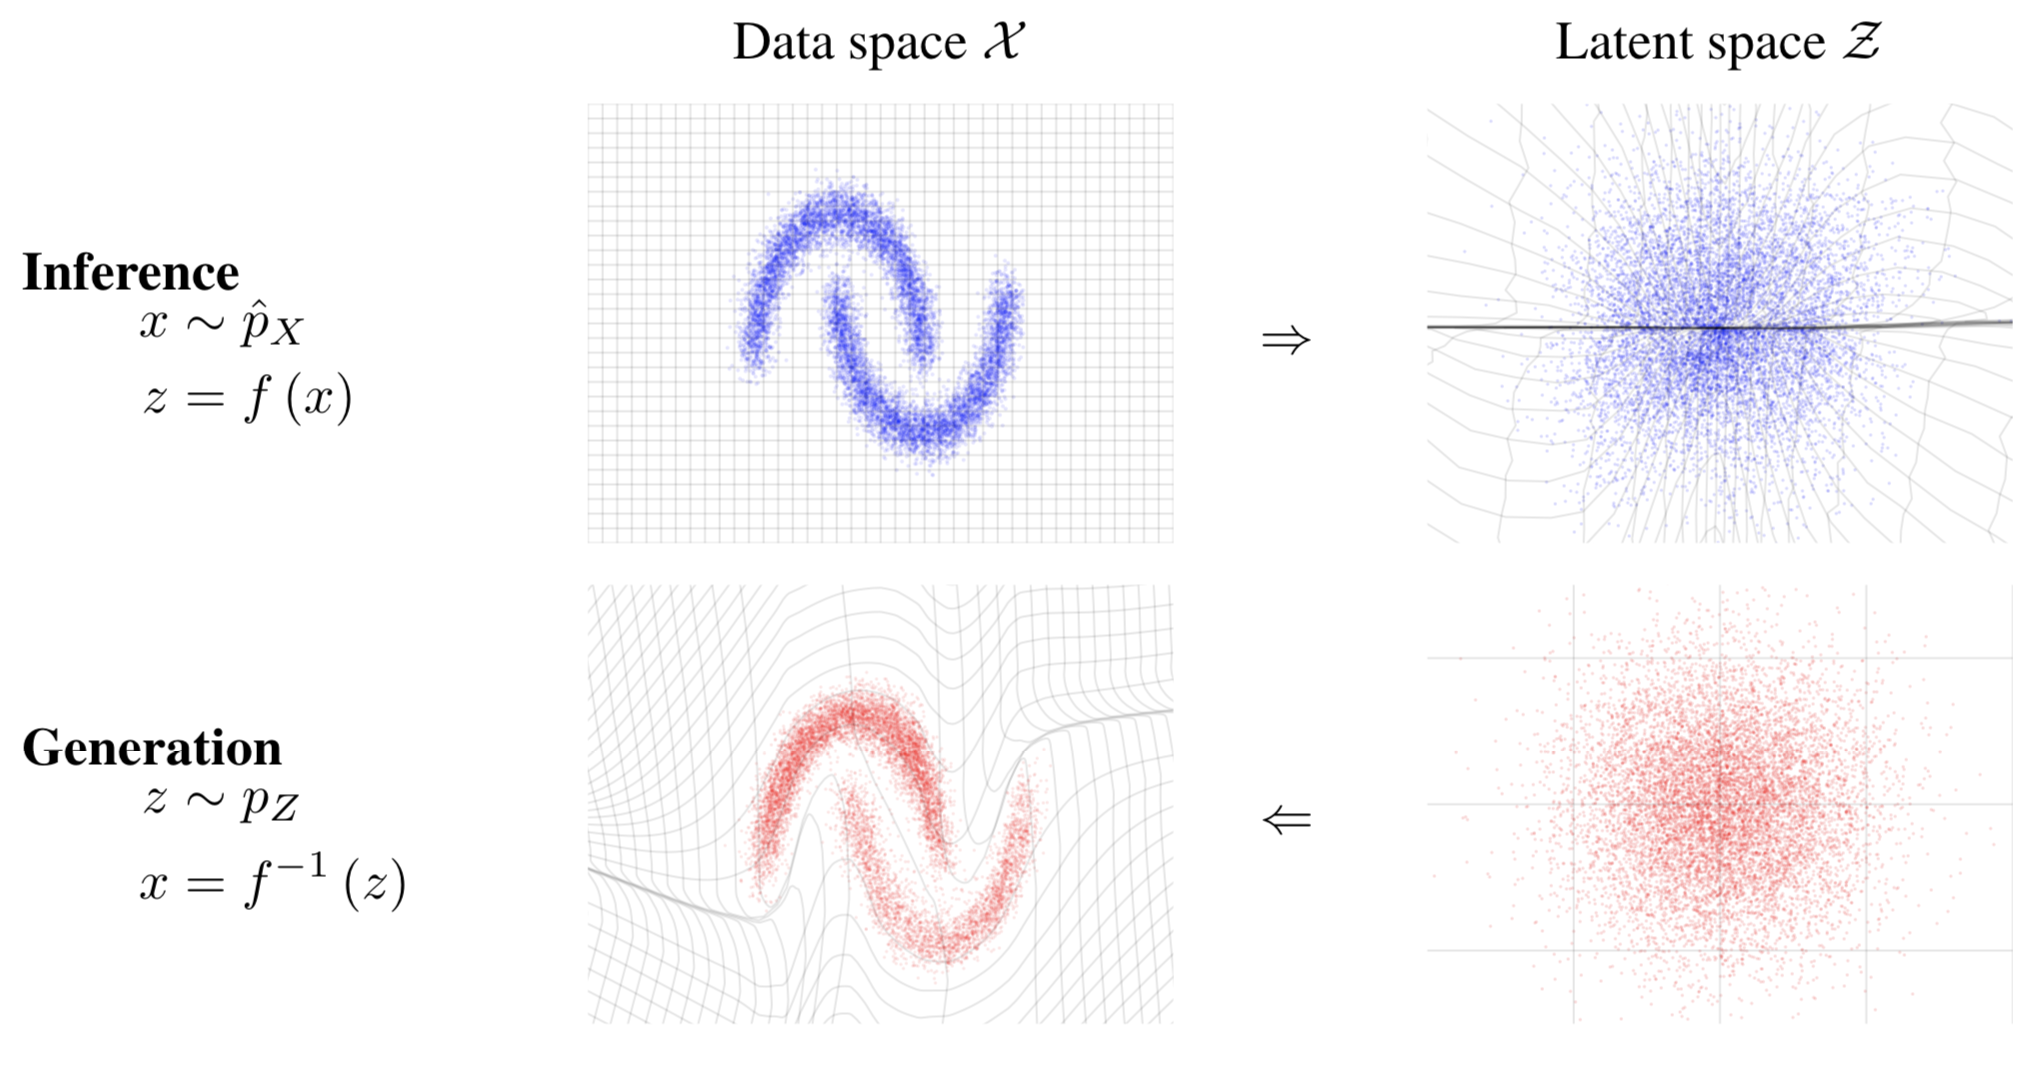
\includegraphics[width=0.7\linewidth]{figs/flows_how2.png}
	\end{figure}
	\vspace{-0.3cm}
		\begin{block}{Flow likelihood}
			\vspace{-0.3cm}
			\[
			\log p(\bx|\btheta) = \log p(f(\bx, \btheta)) + \log \left|\det \left( \frac{\partial f(\bx, \btheta)}{\partial \bx} \right) \right|
			\]
			\vspace{-0.5cm}
		\end{block}
		\begin{block}{What we want}
			\begin{itemize}
				\item Efficient computation of Jacobian $\frac{\partial f(\bx, \btheta)}{\partial \bx}$;
				\item Efficient sampling from the base distribution $p(\bz)$;
				\item Efficient inversion of $f(\bx, \btheta)$.
			\end{itemize}
			
		\end{block}
	\myfootnotewithlink{https://arxiv.org/abs/1605.08803}{Dinh L., Sohl-Dickstein J., Bengio S. Density estimation using Real NVP, 2016} 
\end{frame}
%=======
\begin{frame}{Planar Flows}
	\vspace{-0.2cm}
	\[
	g(\bz, \btheta) = \bz + \mathbf{u} \, h(\bw^T\bz + b).
	\]
	\vspace{-0.2cm}
	\begin{itemize}
		\item $\btheta = \{\bu, \bw, b\}$;
		\item $h$ is a smooth element-wise non-linearity.
	\end{itemize}
	\begin{align*}
		\left| \det \left( \frac{\partial g(\bz, \btheta)}{\partial \bz} \right)\right| &= \left| \det \left( \bI +  h'(\bw^T \bz + b) \bw\bu^T\right) \right| \\
		&= \left| 1 + h'(\bw^T \bz + b) \bw^T \bu \right|
	\end{align*}
	The transformation is invertible, for example, if
	\[
	h = \tanh; \quad h'(\bw^T \bz + b) \bu^T \bw \geq -1.
	\]
	\vspace{-0.3cm}
	\begin{block}{Sylvester flow: planar flow extension}
	\vspace{-0.3cm}
		\[
			g(\bz, \btheta) = \bz + \bA \, h(\bB\bz + \mathbf{b}).
		\]
	\end{block}
	\myfootnote{\href{https://arxiv.org/abs/1505.05770}{Rezende D. J., Mohamed S. Variational Inference with Normalizing Flows, 2015}\\
	\href{https://arxiv.org/abs/1803.05649}{Berg R. et al. Sylvester normalizing flows for variational inference, 2018}}
\end{frame}
%=======
\begin{frame}{Planar Flows}
	\begin{block}{Composition of planar layers}
	\[
		\bz_K = g_1 \circ \dots \circ g_K (\bz); \quad g_k = g(\bz_k, \btheta_k).
	\]
	\end{block}
	\begin{block}{Expressiveness of planar flows}
	\begin{figure}
		\centering
		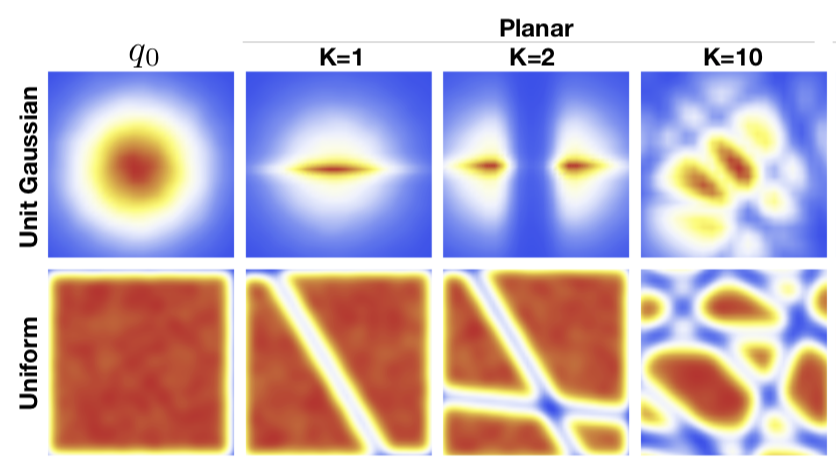
\includegraphics[width=0.8\linewidth]{figs/planar_flows.png}
	\end{figure}
	\end{block}
	\myfootnotewithlink{https://arxiv.org/abs/1505.05770}{Rezende D. J., Mohamed S. Variational Inference with Normalizing Flows, 2015} 
\end{frame}
%=======
\begin{frame}{Jacobian structure}

	\begin{block}{Flow likelihood}
		\[
		\log p(\bx|\btheta) = \log p(f(\bx, \btheta)) + \log \left|\det \left( \frac{\partial f(\bx, \btheta)}{\partial \bx} \right) \right|
		\]
	\end{block}
	\begin{itemize}
		\item What is a determinant of a diagonal matrix?
		\[
		\bz = f(\bx, \btheta) = (f_1(x_1, \btheta), \dots, f_m(x_m, \btheta)).
		\]
		\[
		\log \left|\det \left( \frac{\partial f(\bx, \btheta)}{\partial \bx} \right) \right| = \log \left| \prod_{i=1}^m f_i'(x_i, \btheta) \right| = \sum_{i=1}^m \log \left| f_i'(x_i, \btheta) \right|.
		\]
		\item What is a determinant of a triangular matrix? \\
		Let $z_i$ depend only on $\bx_{1:i}$ (or without loss of generality $x_i$ depends on $\bz_{1:i}$). \\
		What is the Jacobian of such a transformation?
	\end{itemize}
\end{frame}
%=======
\begin{frame}{NICE}
	\begin{block}{Coupling layer}
		\vspace{-0.5cm}
		\begin{equation*}
			\begin{cases} \bz_{1:d} = \bx_{1:d} \\ \bz_{d:m} = \tau (\bx_{d:m}, c(\bx_{1:d}))\end{cases} \quad 
			\begin{cases} \bx_{1:d} = \bz_{1:d} \\ \bx_{d:m} = \tau^{-1} (\bz_{d:m}, c(\bz_{1:d}))\end{cases}
		\end{equation*}
		\vspace{-0.3cm}
		\begin{itemize}
			\item $c: \mathbb{R}^d \rightarrow \mathbb{R}^{k}$ -- coupling function (do not need to be invertible);
			\item $\tau : \mathbb{R}^{m - d} \times c(\mathbb{R}^d) \rightarrow \mathbb{R}^{m - d}$ -- coupling law.
			\item 
			\[
			\det \left( \frac{\partial \bz}{\partial \bx} \right) = \det 
			\begin{pmatrix}
				\bI_d & 0_{d \times m - d} \\
				\frac{\partial \bz_{d:m}}{\partial \bx_{1:d}} & \frac{\partial \bz_{d:m}}{\partial \bx_{d:m}}
			\end{pmatrix} = 
			\det \left( \frac{\partial \bz_{d:m}}{\partial \bx_{d:m}} \right)
			\]
		\end{itemize}
	\end{block}
	\vspace{-0.3cm}
	\begin{block}{Coupling function $c(\cdot)$}
		Any complex function (without restrictions). For example, neural network.
	\end{block}
	\myfootnotewithlink{https://arxiv.org/abs/1410.8516}{Dinh L., Krueger D., Bengio Y. NICE: Non-linear Independent Components Estimation, 2014}
\end{frame}
%=======
\begin{frame}{NICE}
	\begin{block}{Coupling layer}
		\vspace{-0.8cm}
		\begin{equation*}
			\begin{cases} \bz_{1:d} = \bx_{1:d}; \\ \bz_{d:m} = \tau (\bx_{d:m}, c(\bx_{1:d}));\end{cases} 
			\quad \Rightarrow \quad 
			\begin{cases} \bx_{1:d} = \bz_{1:d}; \\ \bx_{d:m} = \tau^{-1} (\bz_{d:m}, c(\bz_{1:d})).\end{cases}
		\end{equation*}
		\vspace{-0.5cm}
	\end{block}
	\begin{block}{Coupling law $\tau(\cdot, \cdot)$}
		\begin{itemize}
			\item $\tau(x, c) = x + c$ -- additive;
			\item $\tau(x, c) = x \odot \exp{c_1} + c_2$ -- affine.
		\end{itemize}
	\end{block}
	
	\begin{block}{Jacobian}
			\vspace{-0.3cm}
		\[
		\det \left( \frac{\partial \bz}{\partial \bx} \right) = \det 
		\begin{pmatrix}
			\bI_d & 0_{d \times m - d} \\
			\frac{\partial \bz_{d:m}}{\partial \bx_{1:d}} & \frac{\partial \bz_{d:m}}{\partial \bx_{d:m}}
		\end{pmatrix} = 
		\det \left( \frac{\partial \bz_{d:m}}{\partial \bx_{d:m}} \right)
		\]
	\end{block}
	What is the Jacobian for the additive coupling law? \\
	In this case, the transformation is \textit{volume preserving}.
	
	\myfootnotewithlink{https://arxiv.org/abs/1410.8516}{Dinh L., Krueger D., Bengio Y. NICE: Non-linear Independent Components Estimation, 2014}
\end{frame}
%=======
\begin{frame}{NICE}
	To obtain a more flexible class of distributions, stack more coupling layers (with different ordering of components!). \\
	\begin{block}{Flow samples}
		\begin{figure}
			\centering
			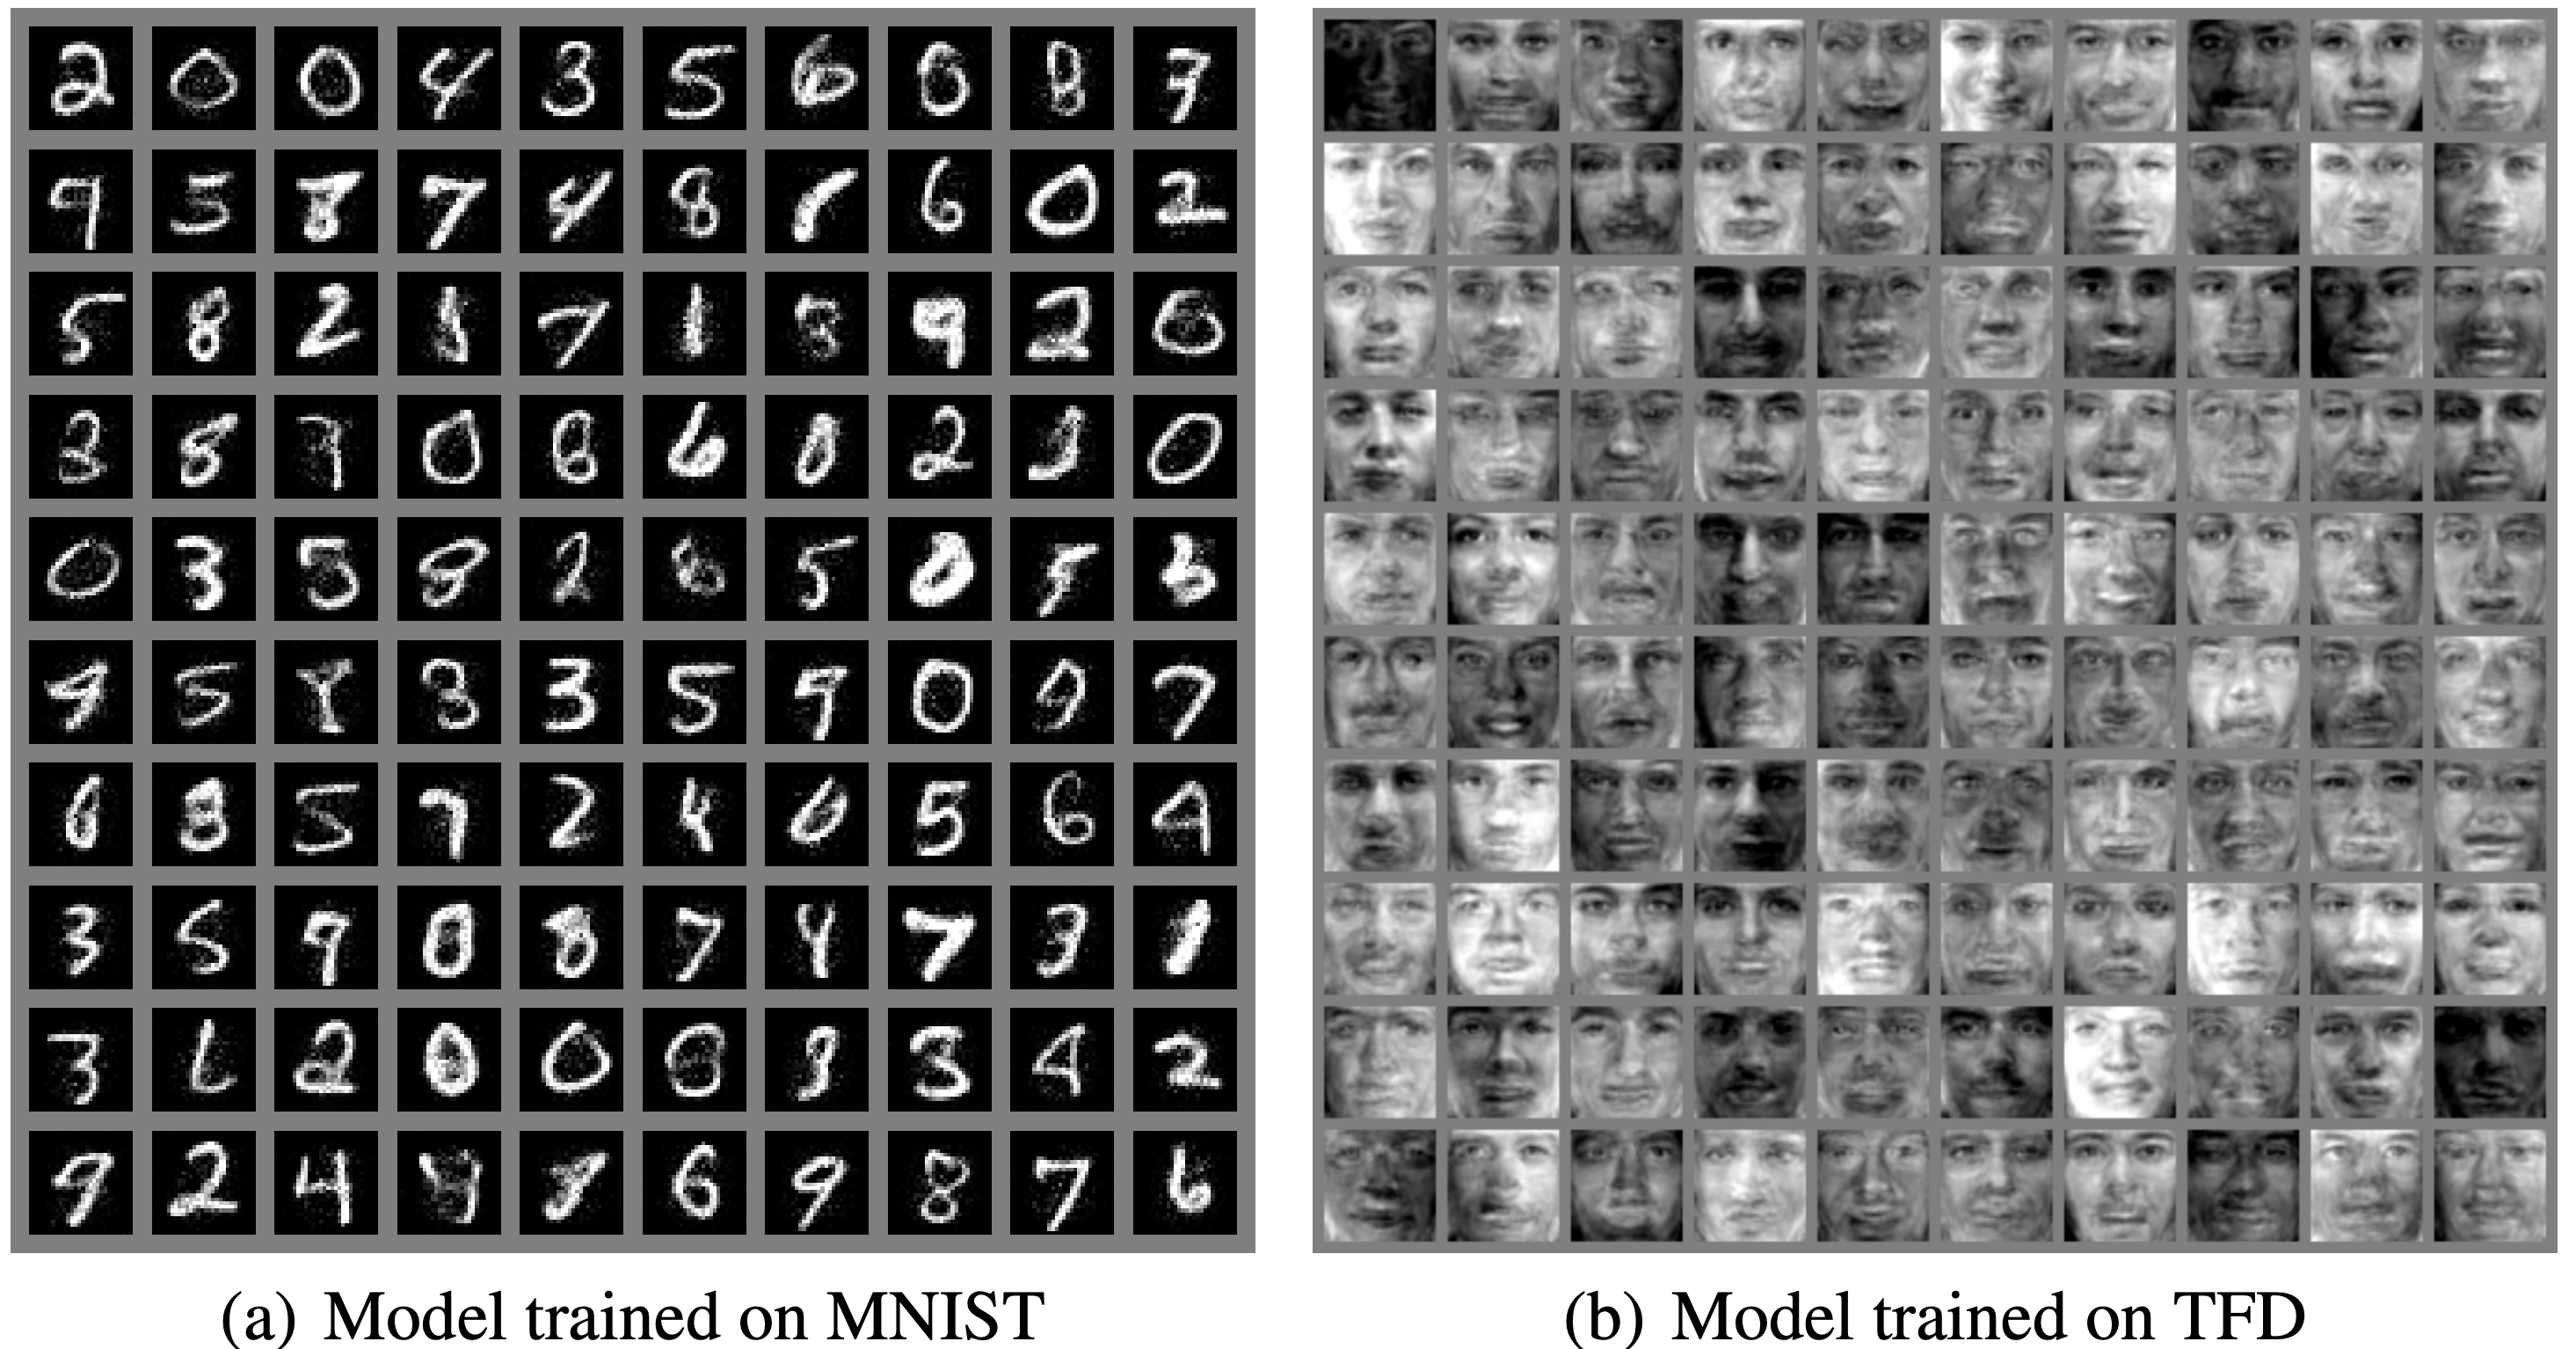
\includegraphics[width=\linewidth]{figs/nice_results.png}
		\end{figure}
	\end{block}
	\myfootnotewithlink{https://arxiv.org/abs/1410.8516}{Dinh L., Krueger D., Bengio Y. NICE: Non-linear Independent Components Estimation, 2014}
\end{frame}
%=======
\begin{frame}{RealNVP}
	\begin{block}{Affine coupling law}
		\[
		\begin{cases} \bz_{1:d} = \bx_{1:d}; \\ \bz_{d:m} = \bx_{d:m} \odot \exp \left(c_1(\bx_{1:d}, \btheta)\right) + c_2(\bx_{1:d}, \btheta).\end{cases} 
		\]
		\[
		\begin{cases} \bx_{1:d} = \bz_{1:d}; \\ \bx_{d:m} = \left(\bz_{d:m} - c_2(\bz_{1:d}, \btheta) \right) \odot \exp(-c_1(\bz_{1:d}, \btheta)).\end{cases}
		\]
	\end{block}
	\begin{block}{Jacobian}
		\vspace{-0.3cm}
		\[
		\det \left( \frac{\partial \bz}{\partial \bx} \right) = \det 
		\begin{pmatrix}
			\bI_d & 0_{d \times m - d} \\
			\frac{\partial \bz_{d:m}}{\partial \bx_{1:d}} & \frac{\partial \bz_{d:m}}{\partial \bx_{d:m}}
		\end{pmatrix} = \prod_{i=1}^{m - d} \exp (c_1(\bx_{1:d}, \btheta)_i).
		\]
		Non-Volume Preserving (the determinant of Jacobian $\neq 0$).
	\end{block}
	
		\myfootnotewithlink{https://arxiv.org/abs/1605.08803}{Dinh L., Sohl-Dickstein J., Bengio S. Density estimation using Real NVP, 2016} 
\end{frame}
%=======
\begin{frame}{RealNVP}
	\begin{block}{Affine coupling law}
		\[
		\begin{cases} \bz_{1:d} = \bx_{1:d}; \\ \bz_{d:m} = \bx_{d:m} \odot \exp \left(c_1(\bx_{1:d}, \btheta)\right) + c_2(\bx_{1:d}, \btheta).\end{cases} 
		\]
	\end{block}
	How to choose variable partitioning for images?
	\begin{figure}
		\centering
		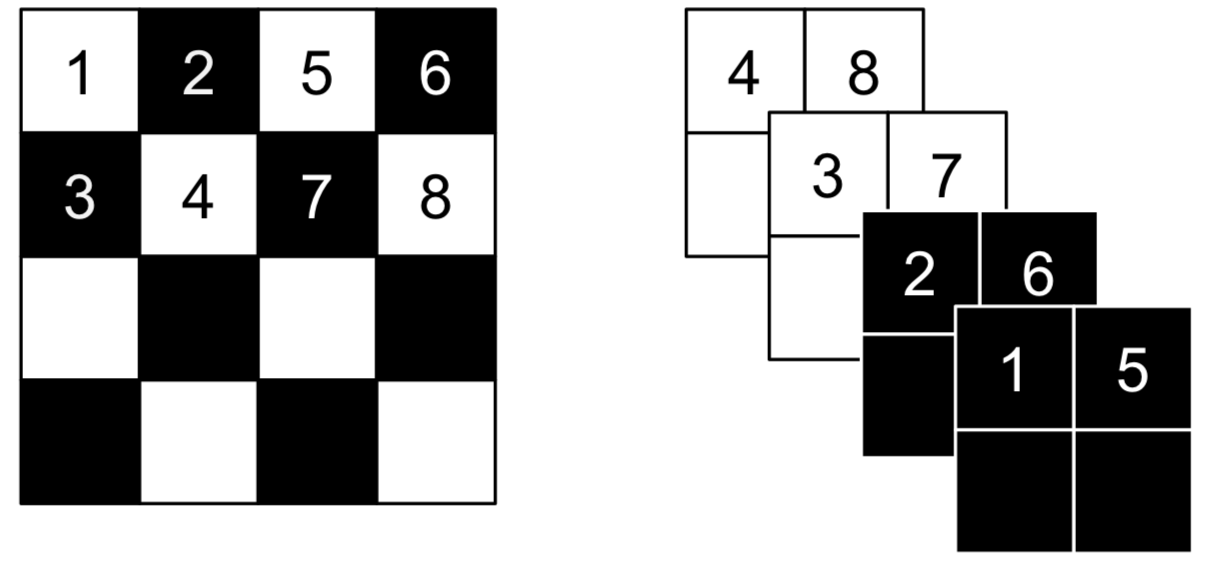
\includegraphics[width=0.75\linewidth]{figs/realnvp_masking.png}
	\end{figure}
	Masked convolutions are used to define ordering.
	
	\myfootnotewithlink{https://arxiv.org/abs/1605.08803}{Dinh L., Sohl-Dickstein J., Bengio S. Density estimation using Real NVP, 2016} 
\end{frame}
%=======
\begin{frame}{RealNVP}
	\begin{block}{Flow samples}
		\begin{figure}
			\centering
			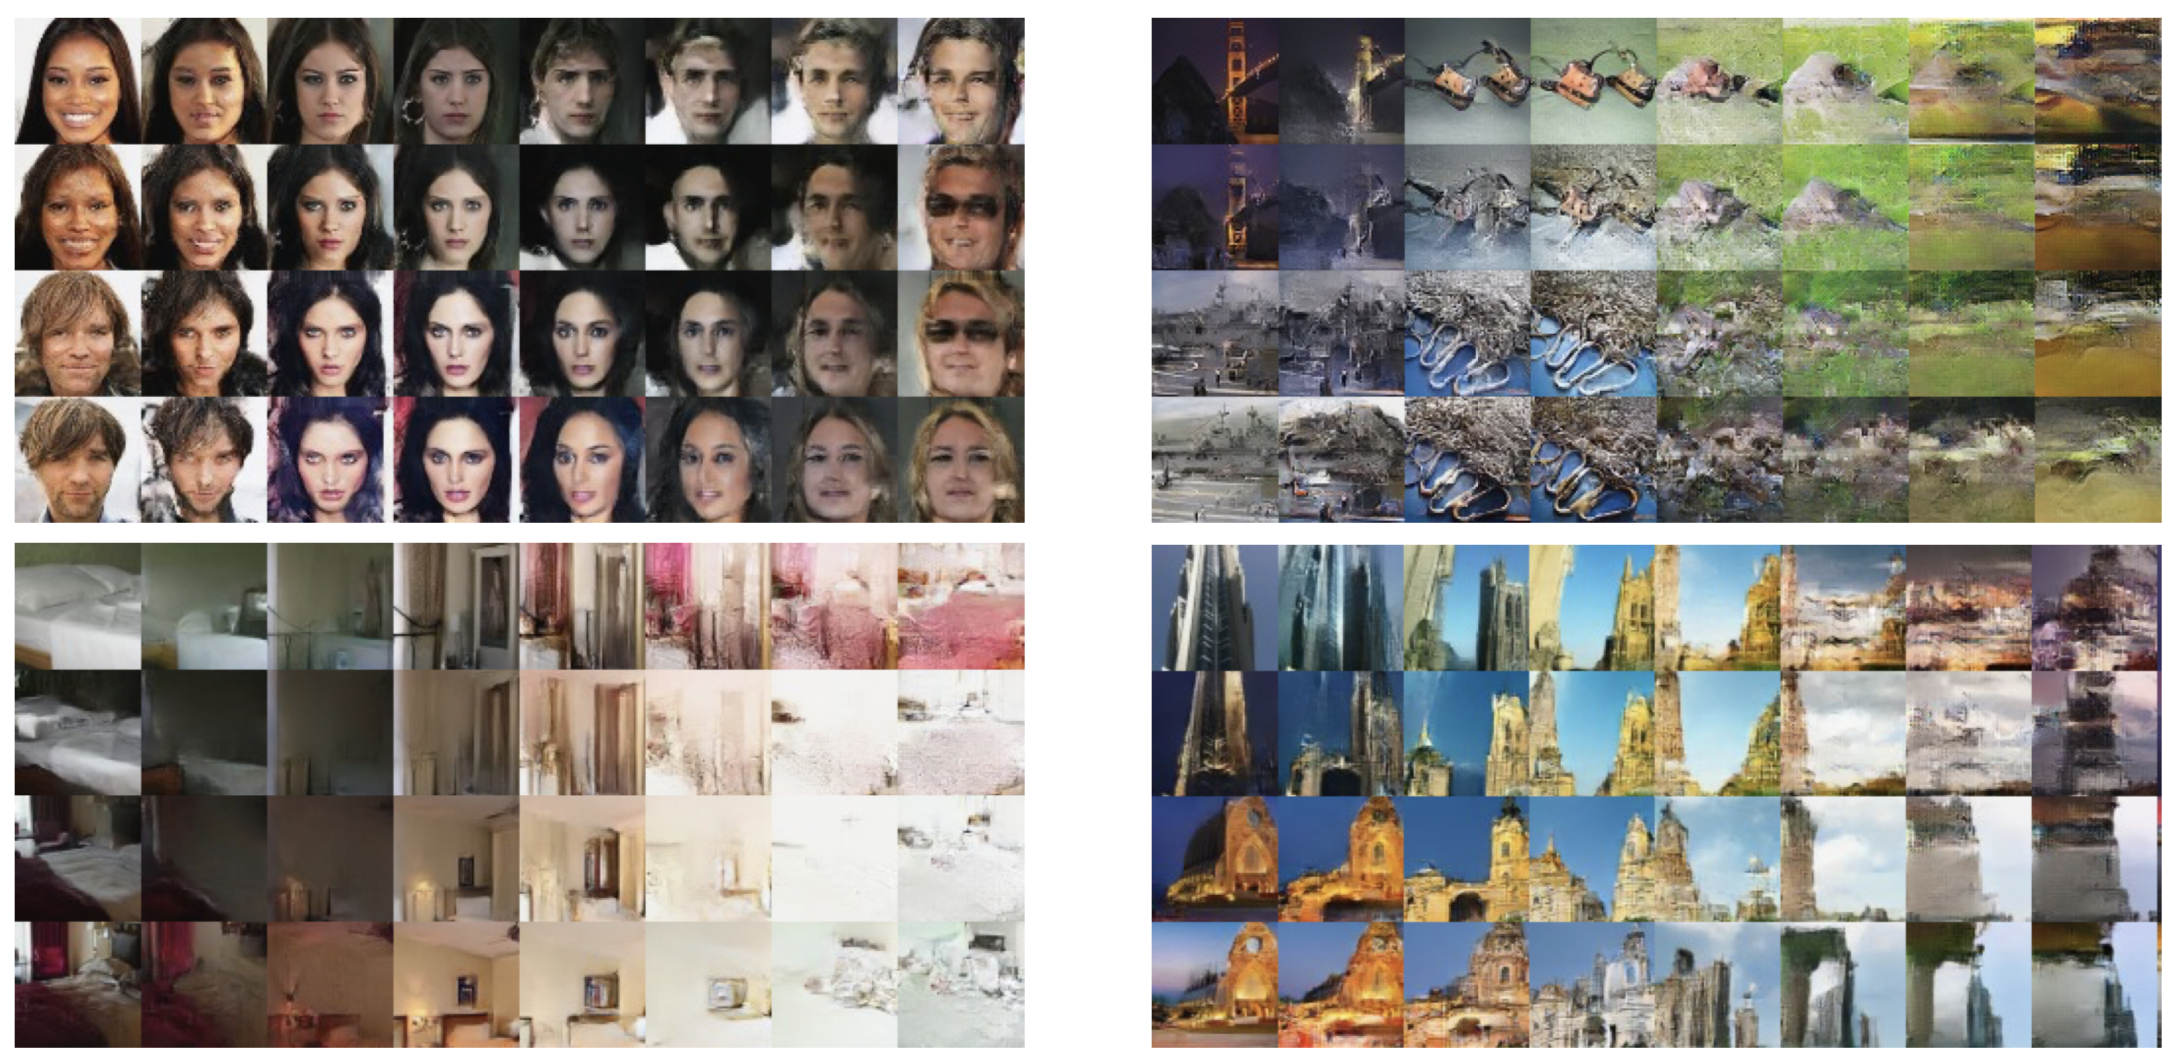
\includegraphics[width=\linewidth]{figs/realnvp_output.png}
		\end{figure}
	\end{block}
	\myfootnotewithlink{https://arxiv.org/abs/1605.08803}{Dinh L., Sohl-Dickstein J., Bengio S. Density estimation using Real NVP, 2016} 
\end{frame}
%=======
\begin{frame}{Glow, 2018}
	\begin{figure}
		\centering
		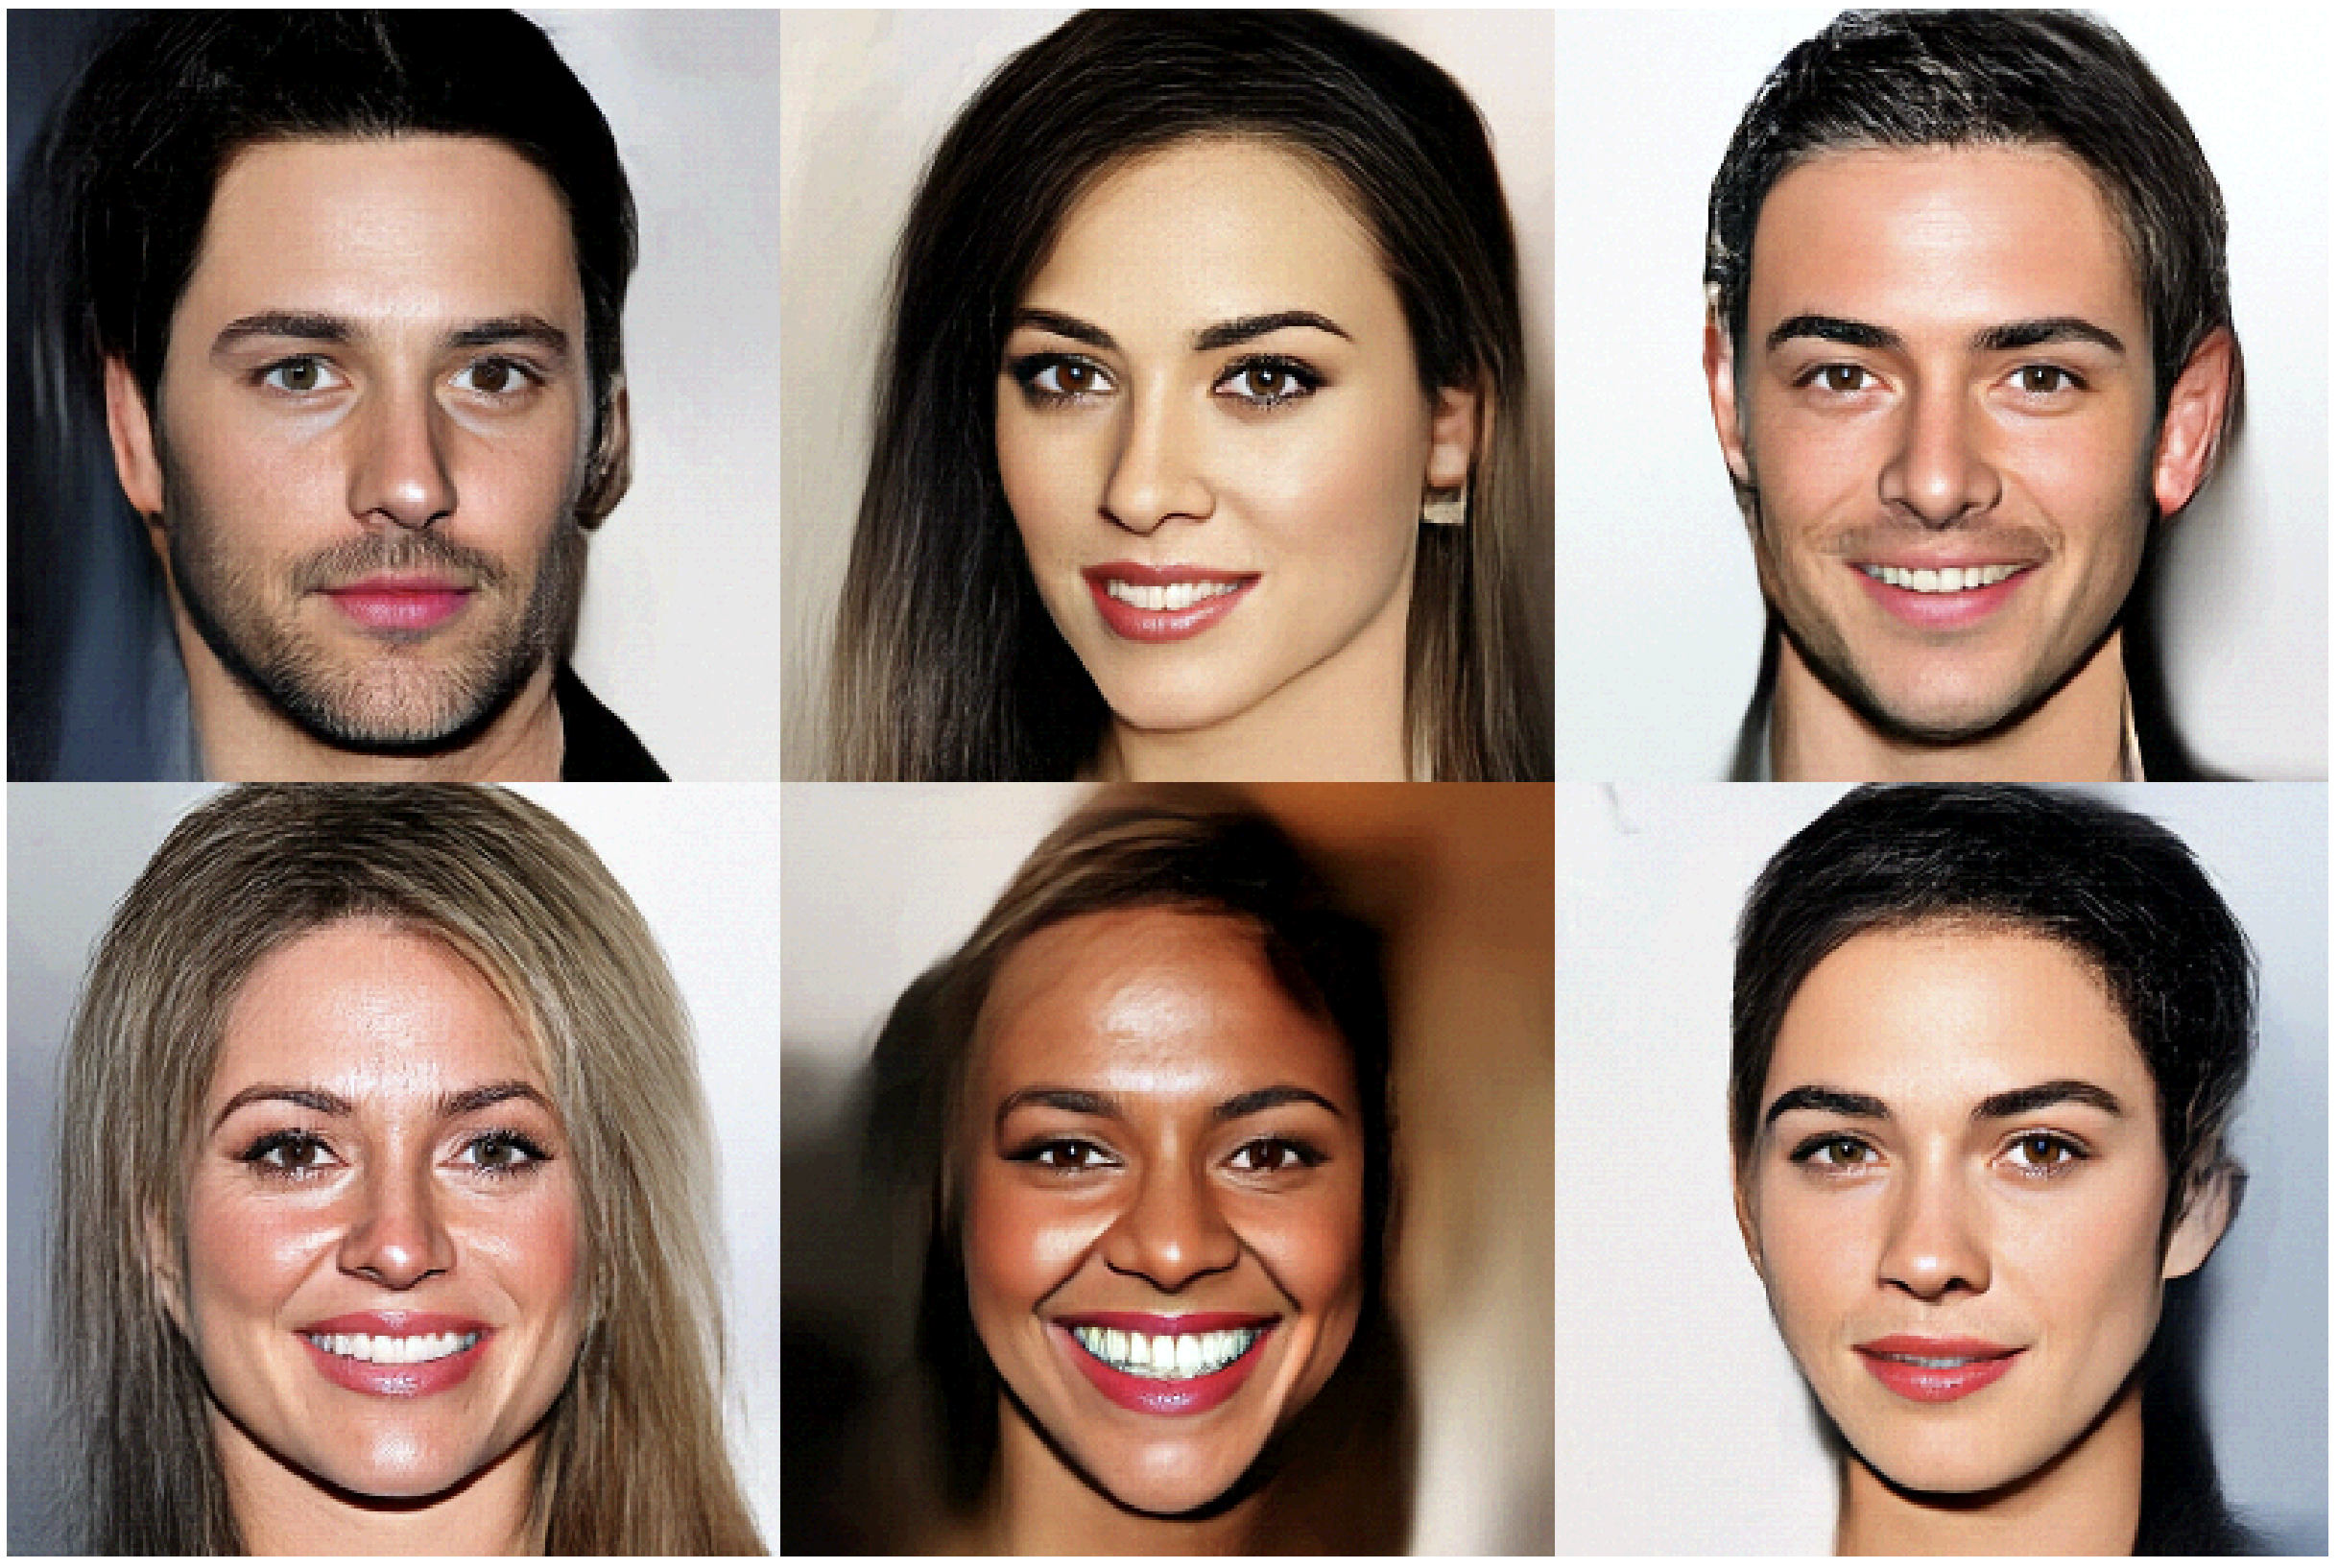
\includegraphics[width=\linewidth]{figs/glow_faces.png}
	\end{figure}
	\myfootnotewithlink{https://arxiv.org/abs/1807.03039}{Kingma D. P., Dhariwal P. Glow: Generative Flow with Invertible 1x1 Convolutions, 2018}
\end{frame}
%=======
\begin{frame}{Glow, 2018}
	\begin{block}{Model architecture}
		\begin{figure}
			\centering
			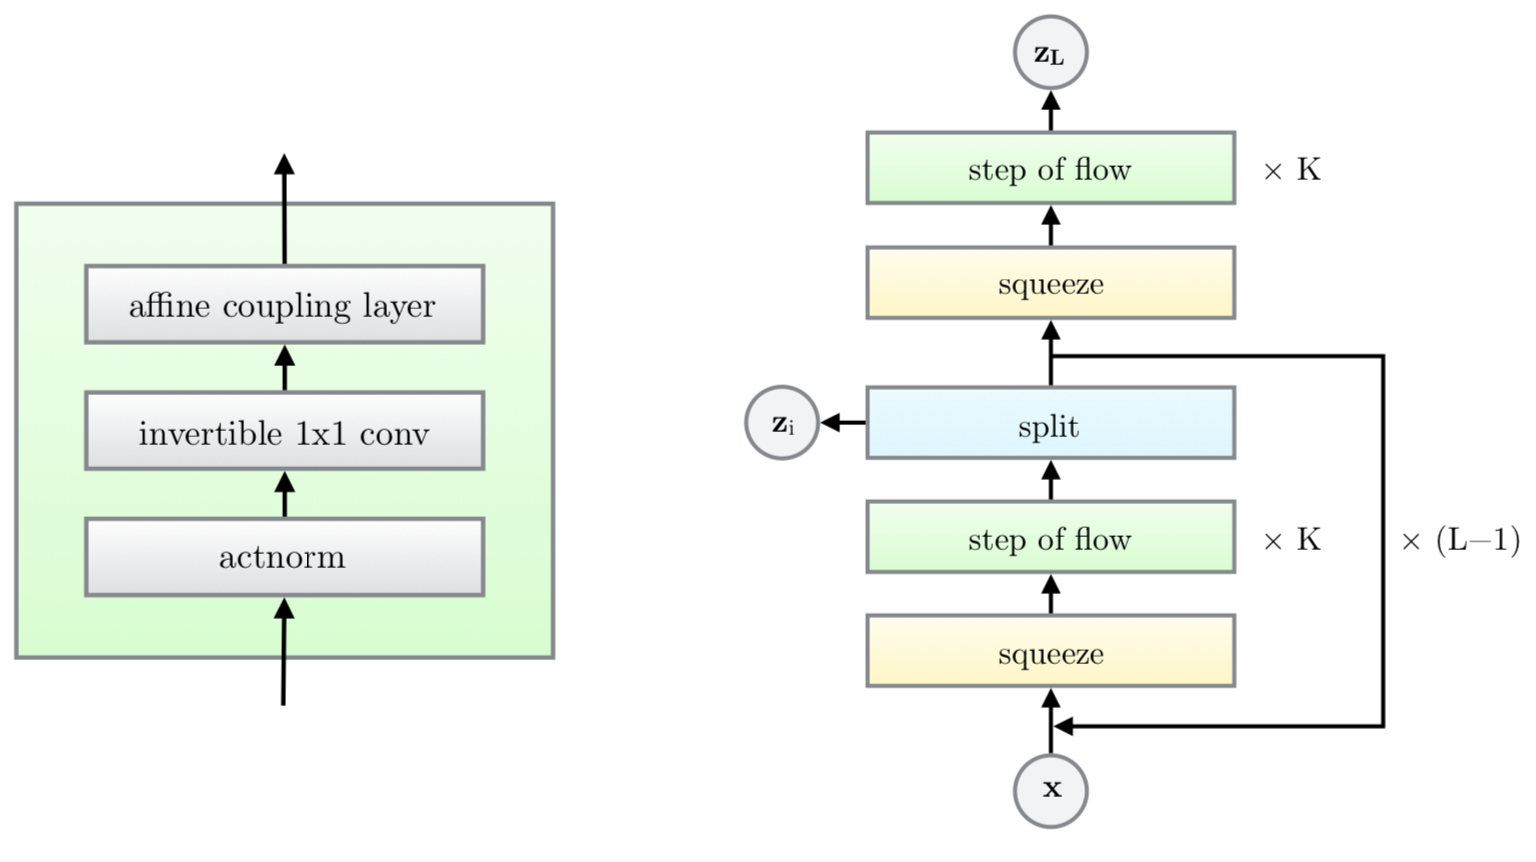
\includegraphics[width=0.8\linewidth]{figs/glow_block.png}
		\end{figure}
	\end{block}
	\vspace{-0.5cm}
	\begin{itemize}
	\item Affine coupling layer (already known).
	\item Invertible 1x1 conv (contribution).
	\item Actnorm (architectural detail).
	\end{itemize}
	\myfootnotewithlink{https://arxiv.org/abs/1807.03039}{Kingma D. P., Dhariwal P. Glow: Generative Flow with Invertible 1x1 Convolutions, 2018}
\end{frame}
%=======
\begin{frame}{Glow, 2018}
	
	\begin{block}{NICE}
		\vspace{-0.2cm}
		\begin{equation*}
			\begin{cases} \bz_1 = \bx_1; \\ \bz_2 = \bx_2 + \mathcal{F}(\bx_1, \btheta);\end{cases}  \quad \Leftrightarrow \quad 
			\begin{cases} \bx_1 = \bz_1; \\ \bx_2 = \bz_2 - \mathcal{F}(\bz_1, \btheta).\end{cases} 
		\end{equation*}
		\vspace{-0.2cm}
	\end{block}
	\begin{itemize}
	\item First step is a \textbf{split} operator which decouples a variable into 2 subparts: $\bx_1$ and $\bx_2$ (usualy channel-wise).
	The order of decoupling should be manually changed between layers.
	\item Could we use a more general operator?
	\item Let use a rotation matrix via 1x1 invertible convolution.
	
	$\mathbf{W} \in \mathbb{R}^{c \times c}$ - kernel of 1x1 convolution with $c$ input and $c$ output channels.
	
	The computational complexity of computing or differentiating $\det (\mathbf{W})$ is $O(c^3)$.
	\end{itemize}

	\myfootnotewithlink{https://arxiv.org/abs/1807.03039}{Kingma D. P., Dhariwal P. Glow: Generative Flow with Invertible 1x1 Convolutions, 2018}
\end{frame}
%=======
\begin{frame}{Glow, 2018}
	\begin{block}{Basic flow operations}
		\begin{figure}
			\centering
			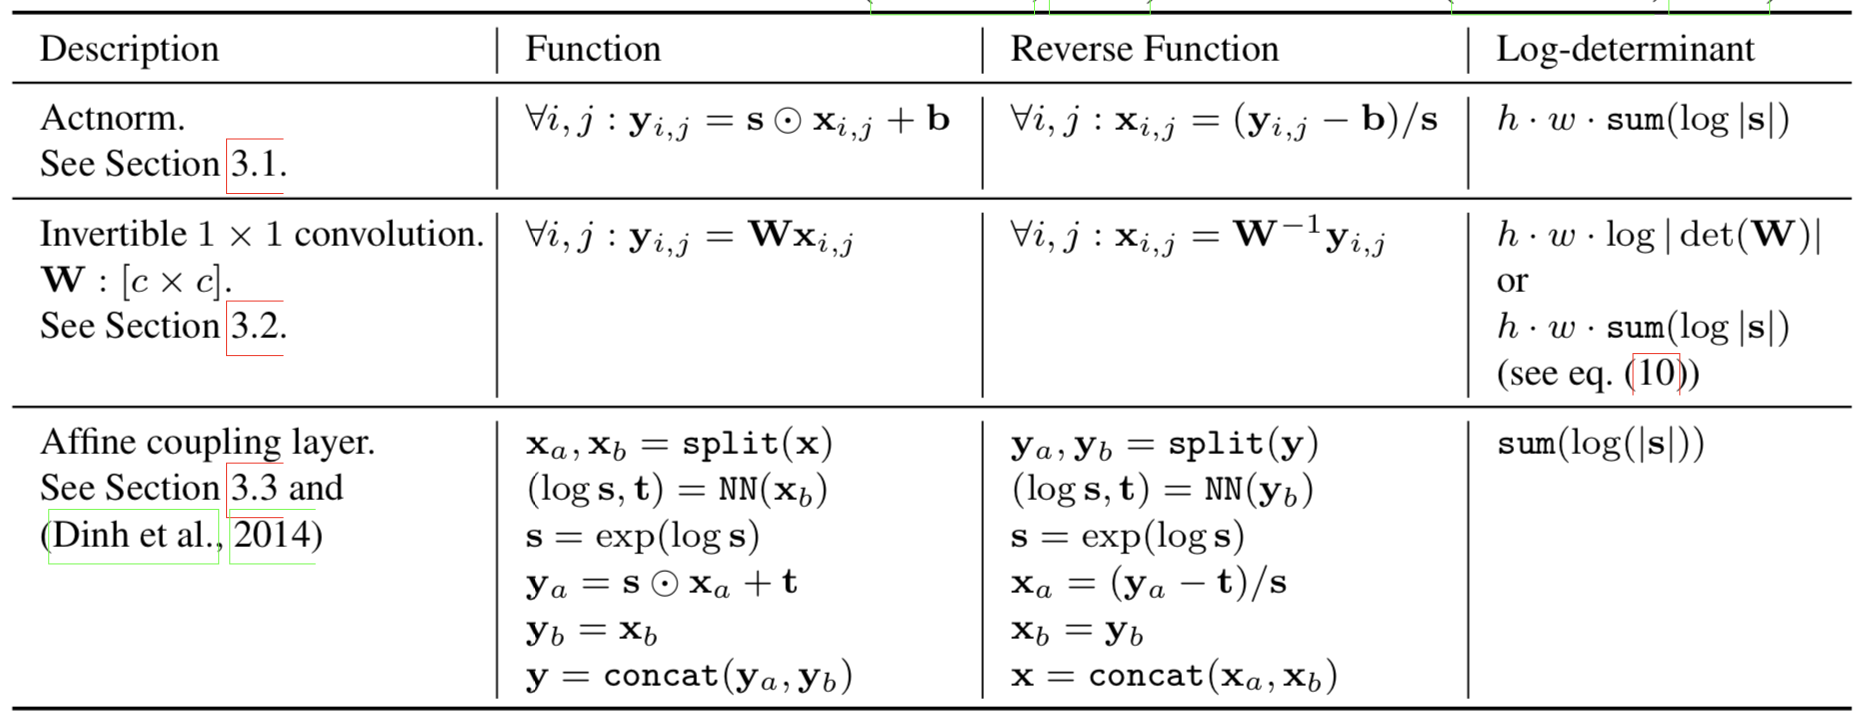
\includegraphics[width=\linewidth]{figs/glow_ops.png}
		\end{figure}
	\end{block}
	\myfootnotewithlink{https://arxiv.org/abs/1807.03039}{Kingma D. P., Dhariwal P. Glow: Generative Flow with Invertible 1x1 Convolutions, 2018}
\end{frame}
%=======
\begin{frame}{Glow, 2018}
	\begin{block}{Invertible 1x1 conv}
		Cost to compute $\det (\mathbf{W})$ is $O(c^3)$. 
		LU-decomposition reduces the cost to $O(c)$:
		\[
		\mathbf{W} = \mathbf{P}\mathbf{L}(\mathbf{U} + \text{diag}(\mathbf{s})),
		\]
		where $\mathbf{P}$ is a permutation matrix, $\mathbf{L}$ is a lower triangular matrix with ones on the diagonal, $\mathbf{U}$ is an
		upper triangular matrix with zeros on the diagonal, and $\mathbf{s}$ is a vector.
	\end{block}
	\begin{figure}
		\centering
		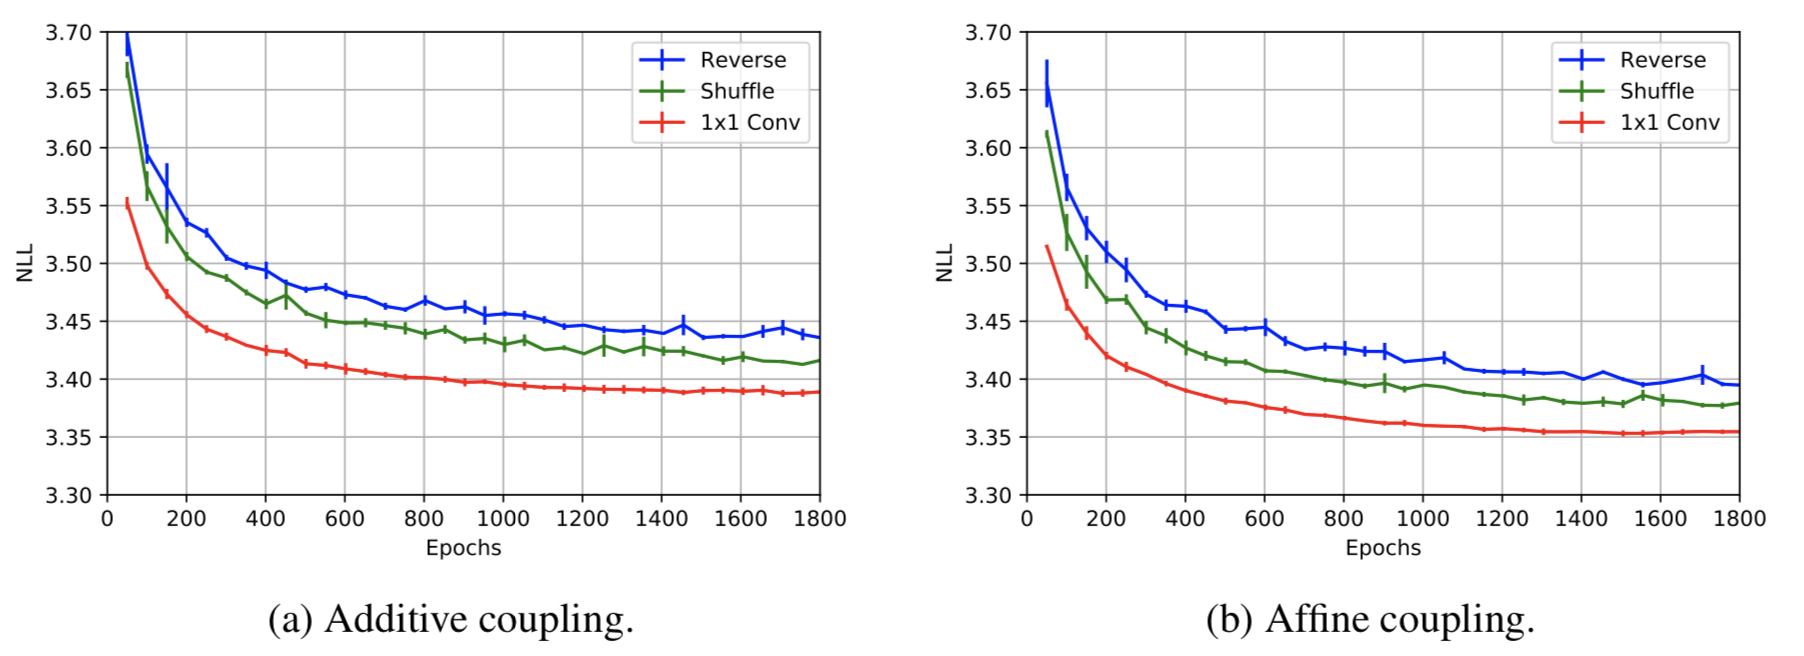
\includegraphics[width=\linewidth]{figs/glow_1x1_conv.png}
	\end{figure}

	\myfootnotewithlink{https://arxiv.org/abs/1807.03039}{Kingma D. P., Dhariwal P. Glow: Generative Flow with Invertible 1x1 Convolutions, 2018}  
\end{frame}
%=======
\begin{frame}{Glow, 2018}
	\begin{block}{Face interpolation}
		\vspace{-0.3cm}
		\begin{figure}
			\centering
			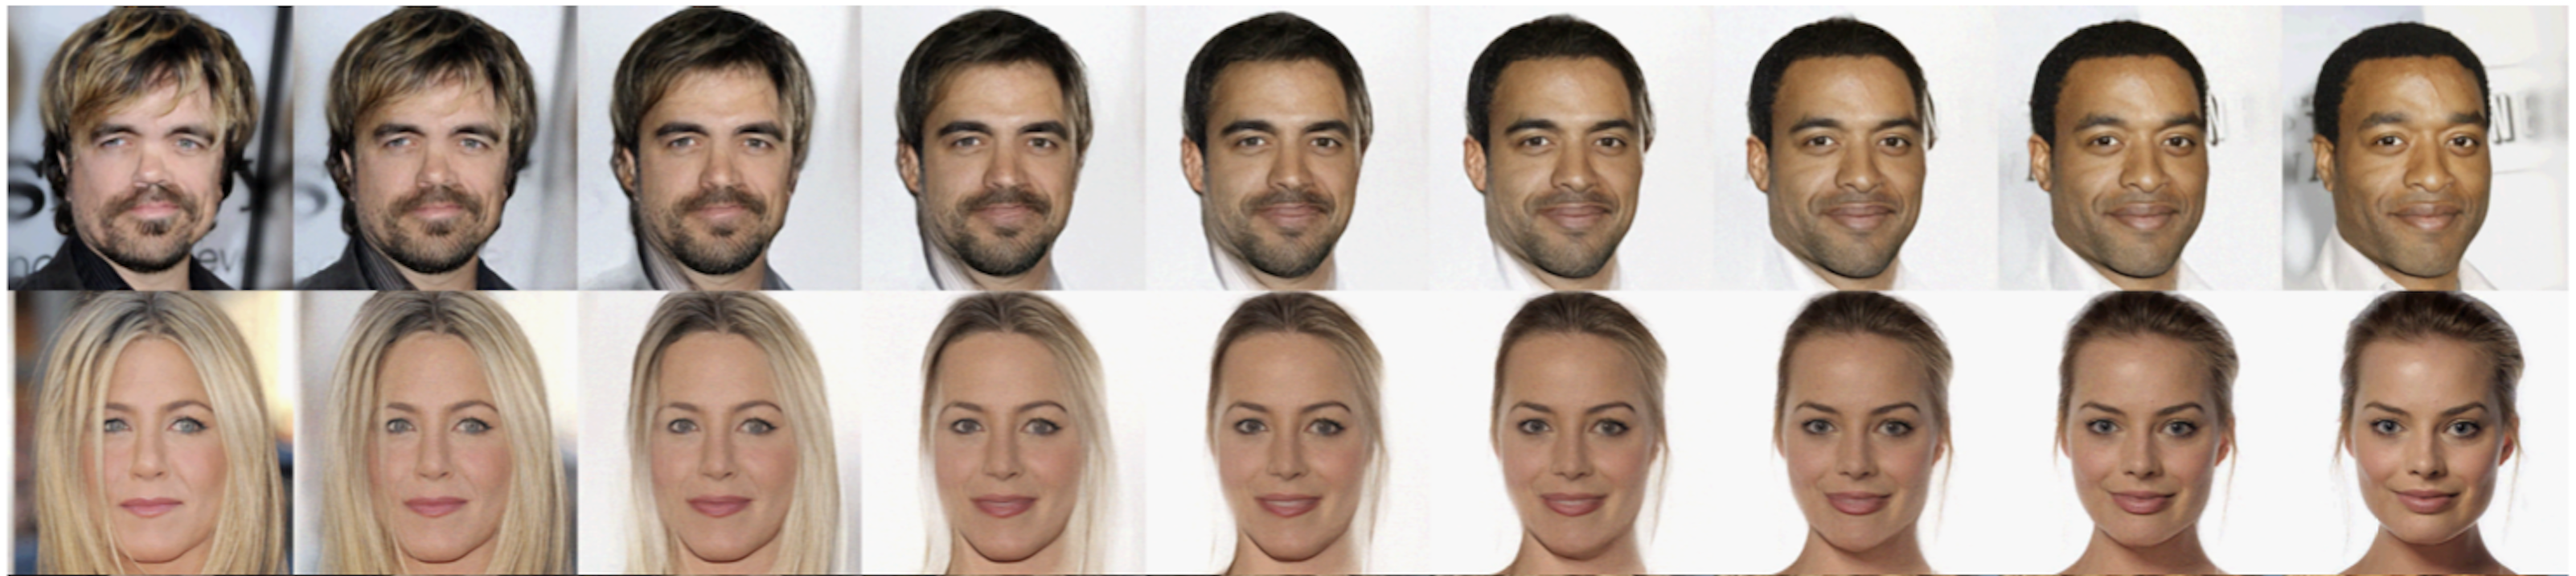
\includegraphics[width=\linewidth]{figs/glow_interpolation.png}
		\end{figure}
		\vspace{-0.3cm}
	\end{block}
	\begin{block}{Face attributes manipulation}
		\begin{figure}
			\centering
			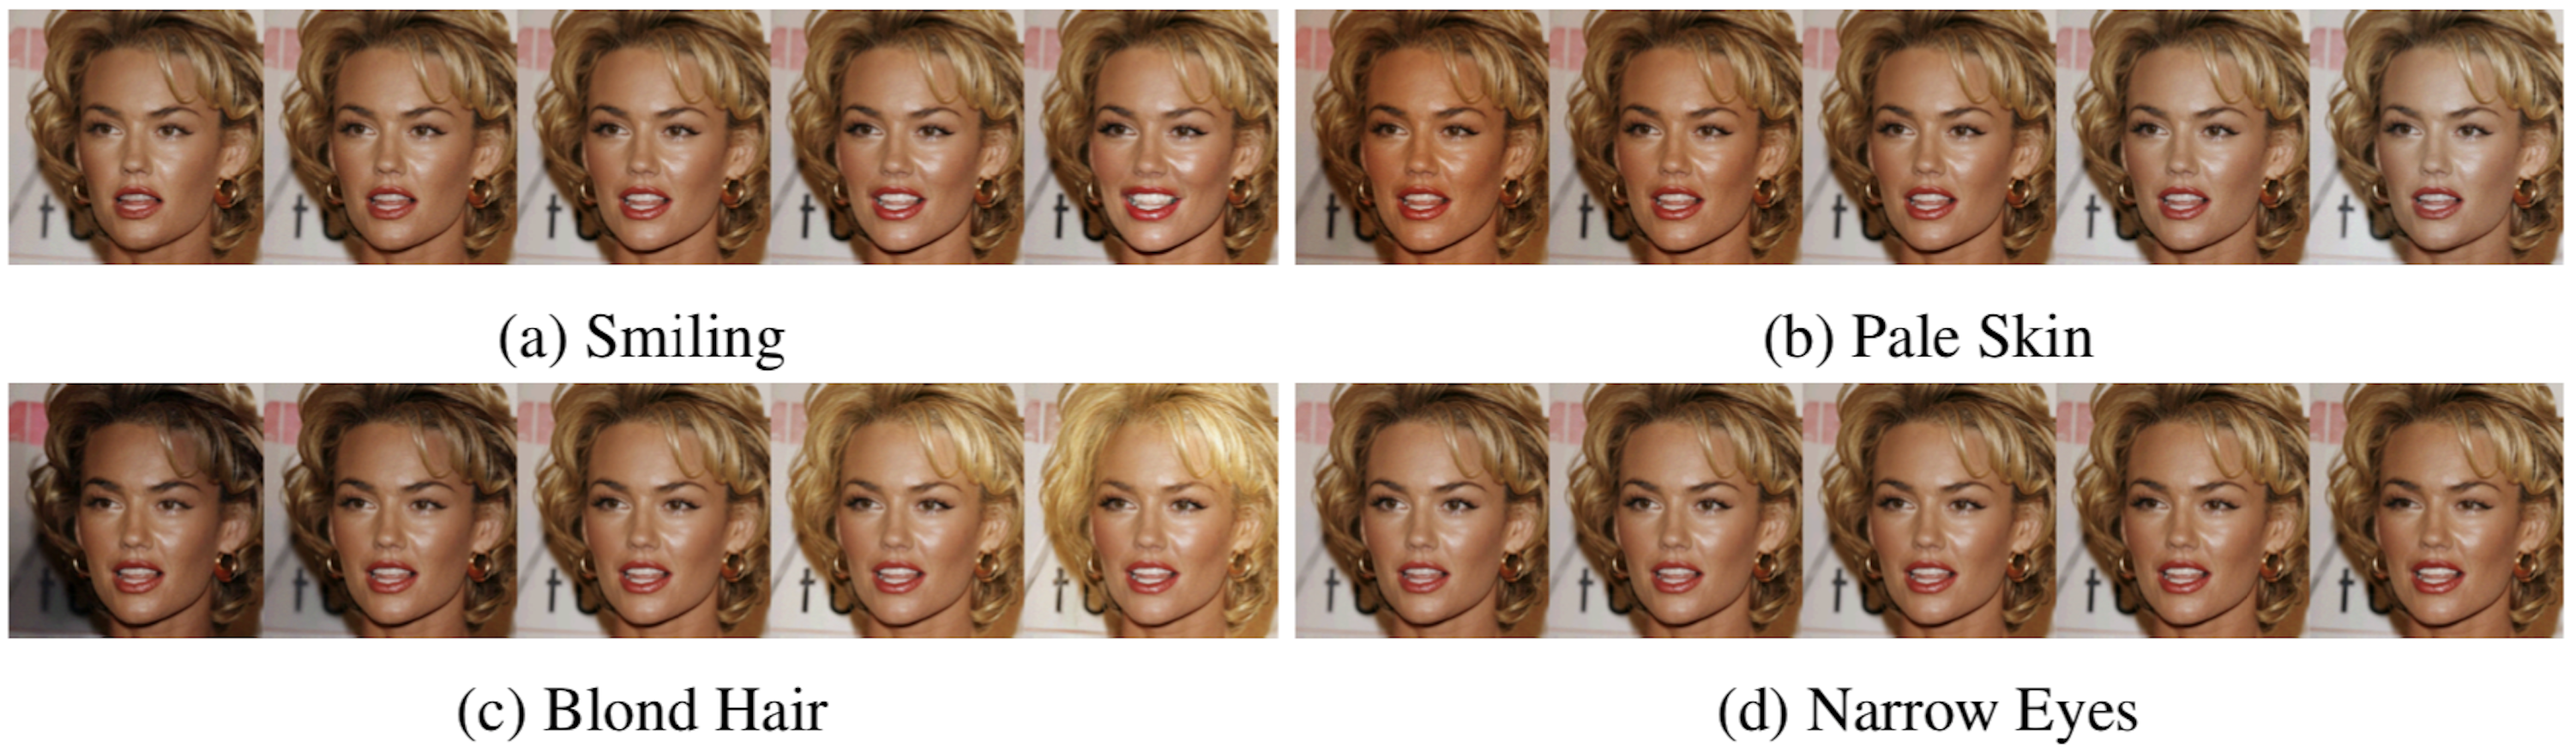
\includegraphics[width=\linewidth]{figs/glow_attributes.png}
		\end{figure}
	\end{block}

	\myfootnotewithlink{https://arxiv.org/abs/1807.03039}{Kingma D. P., Dhariwal P. Glow: Generative Flow with Invertible 1x1 Convolutions, 2018}
\end{frame}
%=======
\begin{frame}{Likelihood-based models}
	\begin{block}{Exact likelihood evaluation}
		\begin{itemize}
			\item Autoregressive models (PixelCNN, WaveNet);
			\item Flow models (NICE, RealNVP, Glow).
		\end{itemize}
	\end{block}
	\begin{block}{Approximate likelihood evaluation}
		\begin{itemize}
			\item Latent variable models (VAE).
		\end{itemize}
	\end{block}
	What are the pros and cons of each of them? \\
	\vspace{0.2cm}
\end{frame}
%=======
\begin{frame}{VAE recap}
	\begin{block}{ELBO}
	\vspace{-0.3cm}
	\[
	\log p(\bx | \btheta) \geq \mathcal{L} (\bphi, \btheta)  = \mathbb{E}_{q(\bz | \bx, \bphi)} \log \frac{p(\bx, \bz | \btheta)}{q(\bz| \bx, \bphi)} \rightarrow \max_{\bphi, \btheta}.
	\]
	\vspace{-0.5cm}
	\end{block}
	\begin{figure}[h]
		\centering
		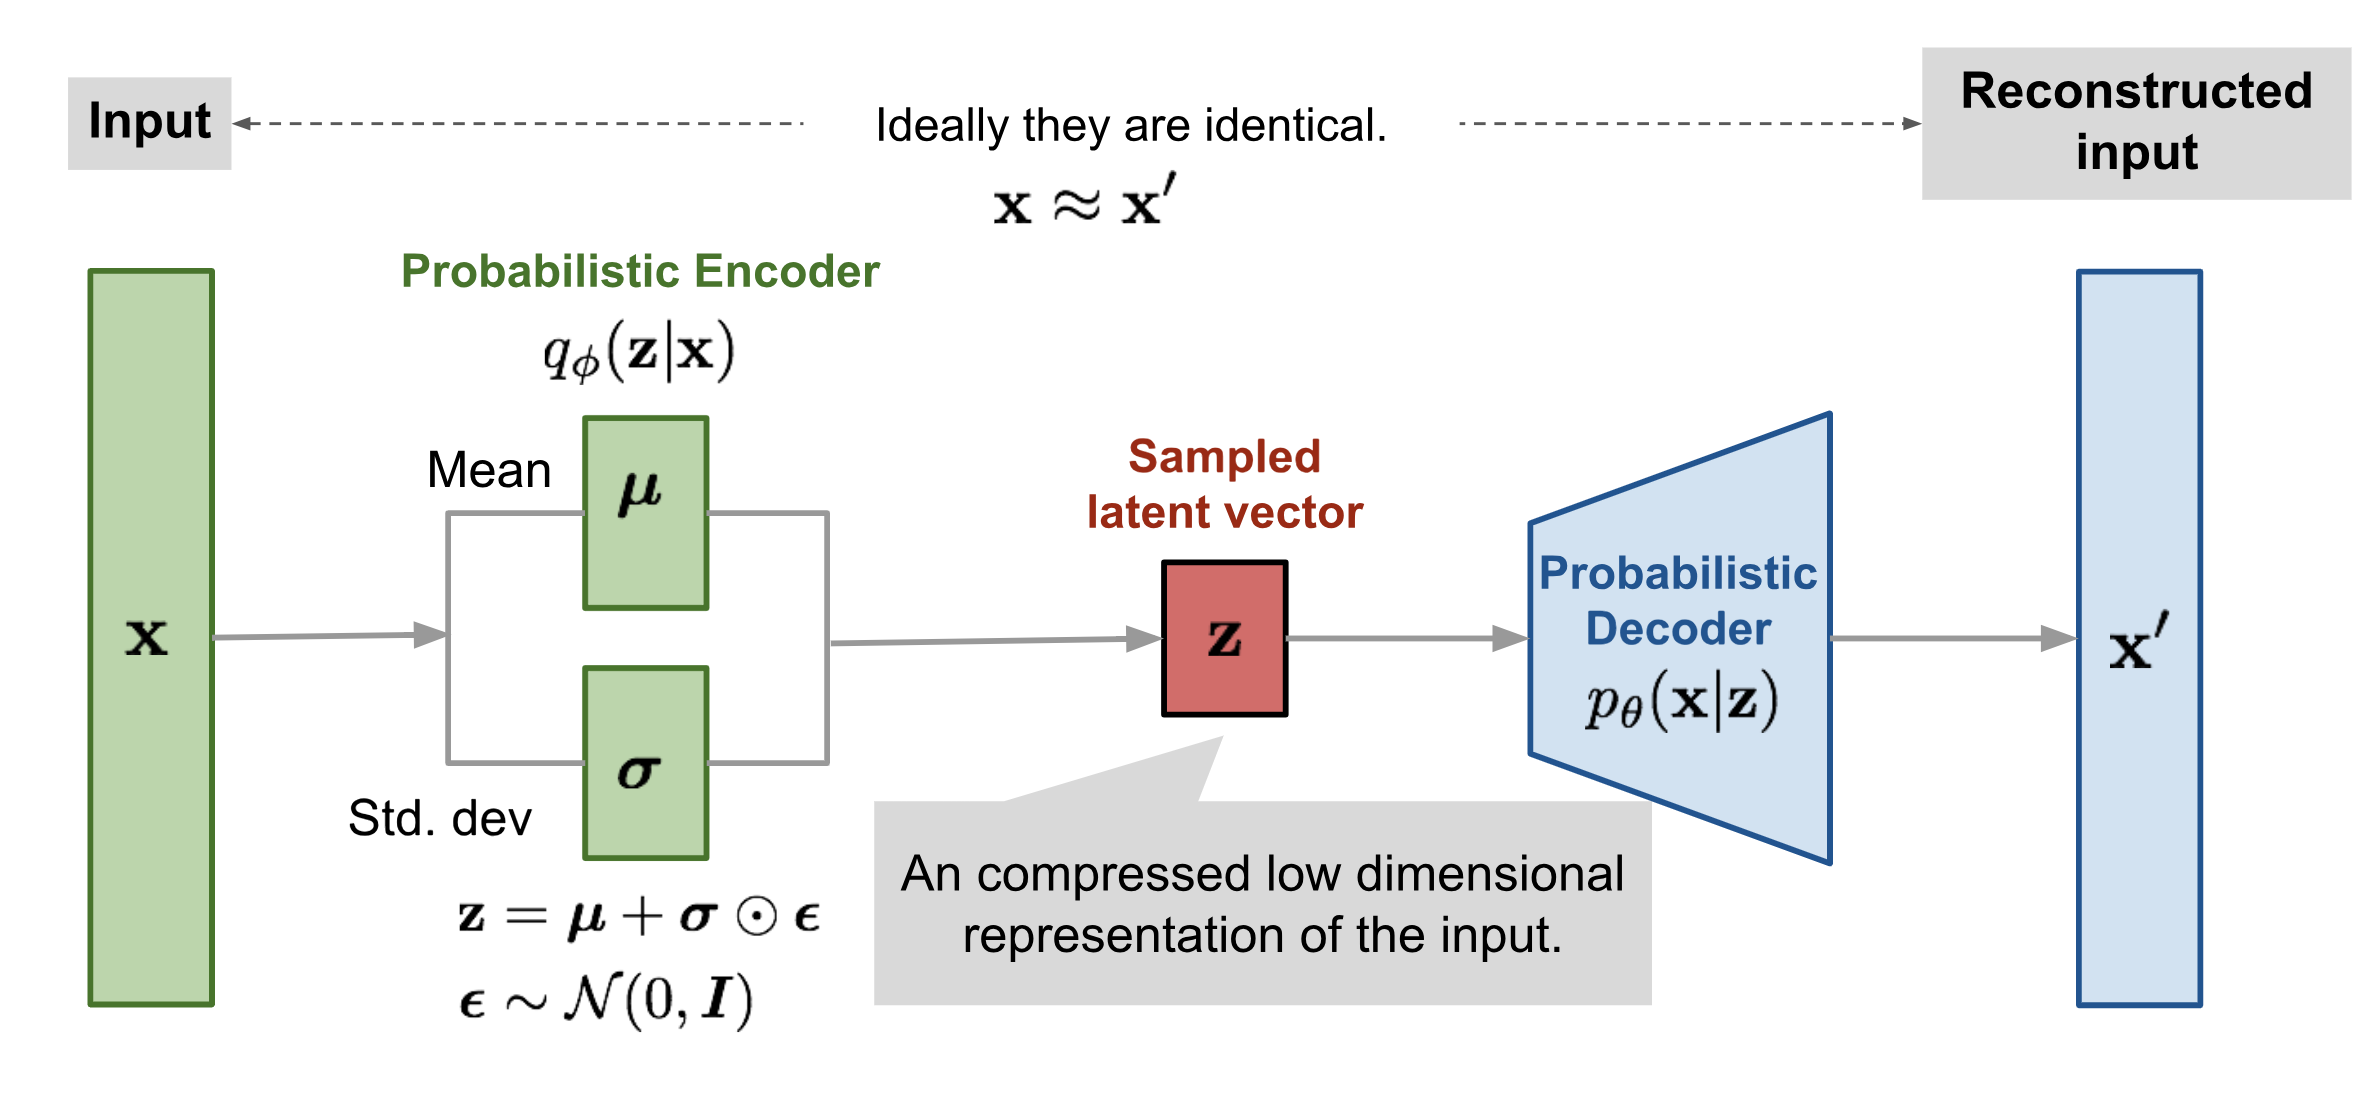
\includegraphics[width=\linewidth]{figs/vae-gaussian.png}
	\end{figure}
	\myfootnotewithlink{https://lilianweng.github.io/lil-log/2018/08/12/from-autoencoder-to-beta-vae.html}{image credit: https://lilianweng.github.io/lil-log/2018/08/12/from-autoencoder-to-beta-vae.html}
	
\end{frame}
%=======
\begin{frame}{VAE limitations}
	\begin{itemize}
		\item Poor variational posterior distribution (encoder)
		\[
		q(\bz | \bx, \bphi) = \mathcal{N}(\bz| \bmu_{\bphi}(\bx), \bsigma^2_{\bphi}(\bx)).
		\]
		\item Poor prior distribution
		\[
		p(\bz) = \mathcal{N}(0, \mathbf{I}).
		\]
		\item Poor probabilistic model (decoder)
		\[
		p(\bx | \bz, \btheta) = \mathcal{N}(\bx| \bmu_{\btheta}(\bz), \bsigma^2_{\btheta}(\bz)) \quad (\text{or } \text{Softmax}(\pi(\bz))).
		\]
		\item Loose lower bound
		\[
		\log p(\bx | \btheta) - \mathcal{L}(q, \btheta) = (?).
		\]
	\end{itemize}
\end{frame}
%=======
\begin{frame}{Variational posterior}
	\begin{block}{ELBO}
	\[
		\log p(\bx | \btheta) = \mathcal{L}(q, \btheta) + KL(q(\bz | \bx, \bphi) || p(\bz | \bx, \btheta)).
	\]
	\end{block}
	\begin{itemize}
		\item In E-step of EM-algorithm we wish $KL(q(\bz | \bx, \bphi) || p(\bz | \bx, \btheta)) = 0$. \\
		(In this case the lower bound is tight $\log p(\bx | \btheta) = \mathcal{L}(q, \btheta)$). \\
		\item Normal variational distribution $q(\bz | \bx, \bphi) = \mathcal{N}(\bz| \bmu_{\bphi}(\bx), \bsigma^2_{\bphi}(\bx))$ is poor (e.g. has only one mode). \\
		\item Flows models convert a simple base distribution to a compex one using invertible transformation with simple Jacobian. How to use flows in VAE?
	\end{itemize}
\end{frame}
%=======
\begin{frame}{Flows in VAE}
	Apply a sequence of transformations to the random variable
	\[
	\bz_0 \sim q(\bz | \bx, \bphi) = \mathcal{N}(\bz| \bmu_{\bphi}(\bx), \bsigma^2_{\bphi}(\bx)).
	\]
	Here, $q(\bz | \bx, \bphi)$ (which is a VAE encoder) plays a role of a base distribution.
	\[
	\bz_0 \xrightarrow{g_1} \bz_1 \xrightarrow{g_2} \dots \xrightarrow{g_K} \bz_K, \quad \bz_K = g(\bz_0), \quad g = g_K \circ \dots \circ g_1.
	\]
	Each $g_k $ is a flow transformation (e.g. planar, coupling layer) parameterized by $\bphi_k$.
	\begin{align*}
		\log q_K(\bz_K | \bx, \bphi, \{\bphi_k\}_{k=1}^K) &= \log q(\bz_0 | \bx, \bphi) \\ &- \sum_{k=1}^K \log \left| \det \left( \frac{\partial g_k(\bz_{k - 1}, \bphi_k)}{\partial \bz_{k-1}} \right) \right|.
	\end{align*}

	\myfootnotewithlink{https://arxiv.org/abs/1505.05770}{Rezende D. J., Mohamed S. Variational Inference with Normalizing Flows, 2015} 
\end{frame}
%=======
\begin{frame}{Flows in VAE}
	\begin{block}{ELBO}
		\vspace{-0.3cm}
		\[
			p(\bx | \btheta) \geq \mathcal{L} (\bphi, \btheta)  = \mathbb{E}_{q(\bz | \bx, \bphi)} \log \frac{p(\bx, \bz | \btheta)}{q(\bz| \bx, \bphi)} \rightarrow \max_{\bphi, \btheta}.
		\]
		\vspace{-0.5cm}
	\end{block}
	\begin{block}{Flow model in latent space}
		\vspace{-0.7cm}
		\[
			\log q_K(\bz_K | \bx, \bphi_*) = \log q(\bz_0 | \bx, \bphi) - \sum_{k=1}^K \log \left| \det \left( \frac{\partial g_k(\bz_{k - 1}, \bphi_k)}{\partial \bz_{k-1}} \right) \right|.
		\]
		\vspace{-0.5cm}
	\end{block}
	Let use $q_K(\bz_K | \bx, \bphi_*), \, \bphi_* = \{\bphi, \bphi_1, \dots, \bphi_K\}$ as a variational distribution. Here $\bphi$~-- encoder parameters, $\{\bphi_k\}_{k=1}^K$~-- flow parameters.
	
	\begin{itemize}
		\item Encoder outputs base distribution $q(\bz_0 | \bx, \bphi)$.
		\item Flow model $\bz_K = g(\bz_0, \{\bphi_k\}_{k=1}^K)$ transforms the base distribution $q(\bz_0 | \bx, \bphi)$ to the distribution $q_K(\bz_K | \bx, \bphi_*)$.
		\item Distribution $q_K(\bz_K | \bx, \bphi_*)$ is used as a variational distribution for ELBO maximization.
	\end{itemize}
	
	\myfootnotewithlink{https://arxiv.org/abs/1505.05770}{Rezende D. J., Mohamed S. Variational Inference with Normalizing Flows, 2015} 
\end{frame}
%=======
\begin{frame}{Flows in VAE}
	\begin{block}{Flow model in latent space}
		\vspace{-0.7cm}
		\[
			\log q_K(\bz_K | \bx, \bphi_*) = \log q(\bz_0 | \bx, \bphi) - \sum_{k=1}^K \log \left| \det \left( \frac{\partial g_k(\bz_{k - 1}, \bphi_k)}{\partial \bz_{k-1}} \right) \right|.
		\]
		\vspace{-0.5cm}
	\end{block}
	\begin{block}{ELBO objective}
		\vspace{-0.5cm}
		\begin{align*}
			\mathcal{L} (\bphi, \btheta)  &= \mathbb{E}_{q_K(\bz_K | \bx, \bphi_*)} \log \frac{p(\bx, \bz_K | \btheta)}{q_K(\bz_K| \bx, \bphi_*)} \\
			&= \mathbb{E}_{q_K(\bz_K | \bx, \bphi_*)} \bigl[\log p(\bx, \bz_K | \btheta) - \log q_K(\bz_K| \bx, \bphi_*) \bigr] \\ 
			&=  \mathbb{E}_{q_K(\bz_K | \bx, \bphi_*)} \log p(\bx | \bz_K, \btheta) - KL (q_K(\bz_K| \bx, \bphi_*) || p(\bz_K)).
		\end{align*}
	\end{block}
	The second term in ELBO is reverse KL divergence. Planar flows was originally proposed for variational inference in VAE.
	\myfootnotewithlink{https://arxiv.org/abs/1505.05770}{Rezende D. J., Mohamed S. Variational Inference with Normalizing Flows, 2015} 
\end{frame}
%=======
\begin{frame}{Flows in VAE}
	\begin{block}{Variational distribution}
		\vspace{-0.5cm}
		\[
			\log q_K(\bz_K | \bx, \bphi_*) = \log q(\bz_0 | \bx, \bphi) - \sum_{k=1}^K \log \left| \det \left( \frac{\partial g_k(\bz_{k - 1}, \bphi_k)}{\partial \bz_{k-1}} \right) \right|.
		\]
		\vspace{-0.5cm}
	\end{block}
	\begin{block}{ELBO objective}
		\vspace{-0.5cm}
		\begin{align*}
			\mathcal{L} (\bphi, \btheta) 
			&= \mathbb{E}_{q_K(\bz_K | \bx, \bphi_*)} \bigl[\log p(\bx, \bz_K | \btheta) - \log q_K(\bz_K| \bx, \bphi_*) \bigr] \\
			&= \mathbb{E}_{q(\bz_0 | \bx, \bphi)} \left. \bigl[\log p(\bx, \bz_K | \btheta) - \log q_K(\bz_K| \bx, \bphi_*) \bigr]\right|_{\bz_K = g(\bz_0, \{\bphi_k\}_{k=1}^K)} \\
			&= \mathbb{E}_{q(\bz_0 | \bx, \bphi)} \bigg[\log p(\bx, \bz_K | \btheta) -  \log q(\bz_0 | \bx, \bphi ) + \\ & \quad  + \sum_{k=1}^K \log \left| \det \left( \frac{\partial g_k(\bz_{k - 1}, \bphi_k)}{\partial \bz_{k-1}} \right) \right| \bigg].
		\end{align*}
	\end{block}
	\myfootnotewithlink{https://arxiv.org/abs/1505.05770}{Rezende D. J., Mohamed S. Variational Inference with Normalizing Flows, 2015} 
\end{frame}
%=======
\begin{frame}{Flows in VAE}
	\begin{block}{Variational distribution}
		\vspace{-0.6cm}
		\[
			\log q_K(\bz_K | \bx, \bphi_*) = \log q(\bz_0 | \bx, \bphi) - \sum_{k=1}^K \log \left| \det \left( \frac{\partial g_k(\bz_{k - 1}, \bphi_k)}{\partial \bz_{k-1}} \right) \right|.
		\]
		\vspace{-0.6cm}
	\end{block}
	\begin{block}{ELBO objective}
		\vspace{-0.7cm}
		\begin{align*}
			\mathcal{L} (\bphi, \btheta) 
			&= \mathbb{E}_{q(\bz_0 | \bx, \bphi)} \bigg[\log p(\bx, \bz_K | \btheta) -  \log q(\bz_0 | \bx, \bphi ) + \\ & \quad  + \sum_{k=1}^K \log \left| \det \left( \frac{\partial g_k(\bz_{k - 1}, \bphi_k)}{\partial \bz_{k-1}} \right) \right| \bigg].
		\end{align*}
		\vspace{-0.5cm}
	\end{block}
	\begin{itemize}
		\item Obtain samples $\bz_0$ from the encoder.
		\item Apply flow model $\bz_K = g(\bz_0, \{\bphi_k\}_{k = 1}^K)$.
		\item Compute likelihood for $\bz_K$ using the decoder, base distribution for $\bz_0$ and the Jacobian.
		\item We do not need inverse flow function, if we use flows in variational inference.
	\end{itemize}
	\myfootnotewithlink{https://arxiv.org/abs/1505.05770}{Rezende D. J., Mohamed S. Variational Inference with Normalizing Flows, 2015} 
\end{frame}
%=======
\begin{frame}{Summary}
\begin{itemize}
	\item Flow models require tractable Jacobian.
	\vfill
	\item Planar flow is a simple form of an invertible flow model (Sylvester flows are their extension). 
	\vfill
	\item The NICE/RealNVP model is a more powerful type of flow that use coupling layers.
	\vfill
	\item Glow model is a first flow model with superior results.
	\vfill
	\item Flows could be used in variational inference to create powerful variational distribution.

\end{itemize}
\end{frame}
\end{document} 